%   Filename    : chapter_4.tex 

\chapter{Results and Discussions/Analyses}

\section{Results}
According to the results of the requirements analysis and methodology, the team was to identify and devise the main features of the web application such as the requestor view of request, tracking, payment, and profile dashboard. For the college secretary view, we identified implementing features such as document request dashboard, history, request status update, office profile, and request file uploading. The cash officer view, however, will consist of pending payments, history of payments, verification of payments, and uploading of original receipt files. Overall, the system will include features of request creation, payment portal, payment verification, document processing, and request tracking. These features were implemented and will be further discussed in their respective sections below.

\subsection{Requestor View}

\subsubsection{Sign in/Sign up and Dashboard}

    \begin{figure}[h]
        \centering 
        \begin{minipage}[c]{0.5\linewidth}
            \centering
            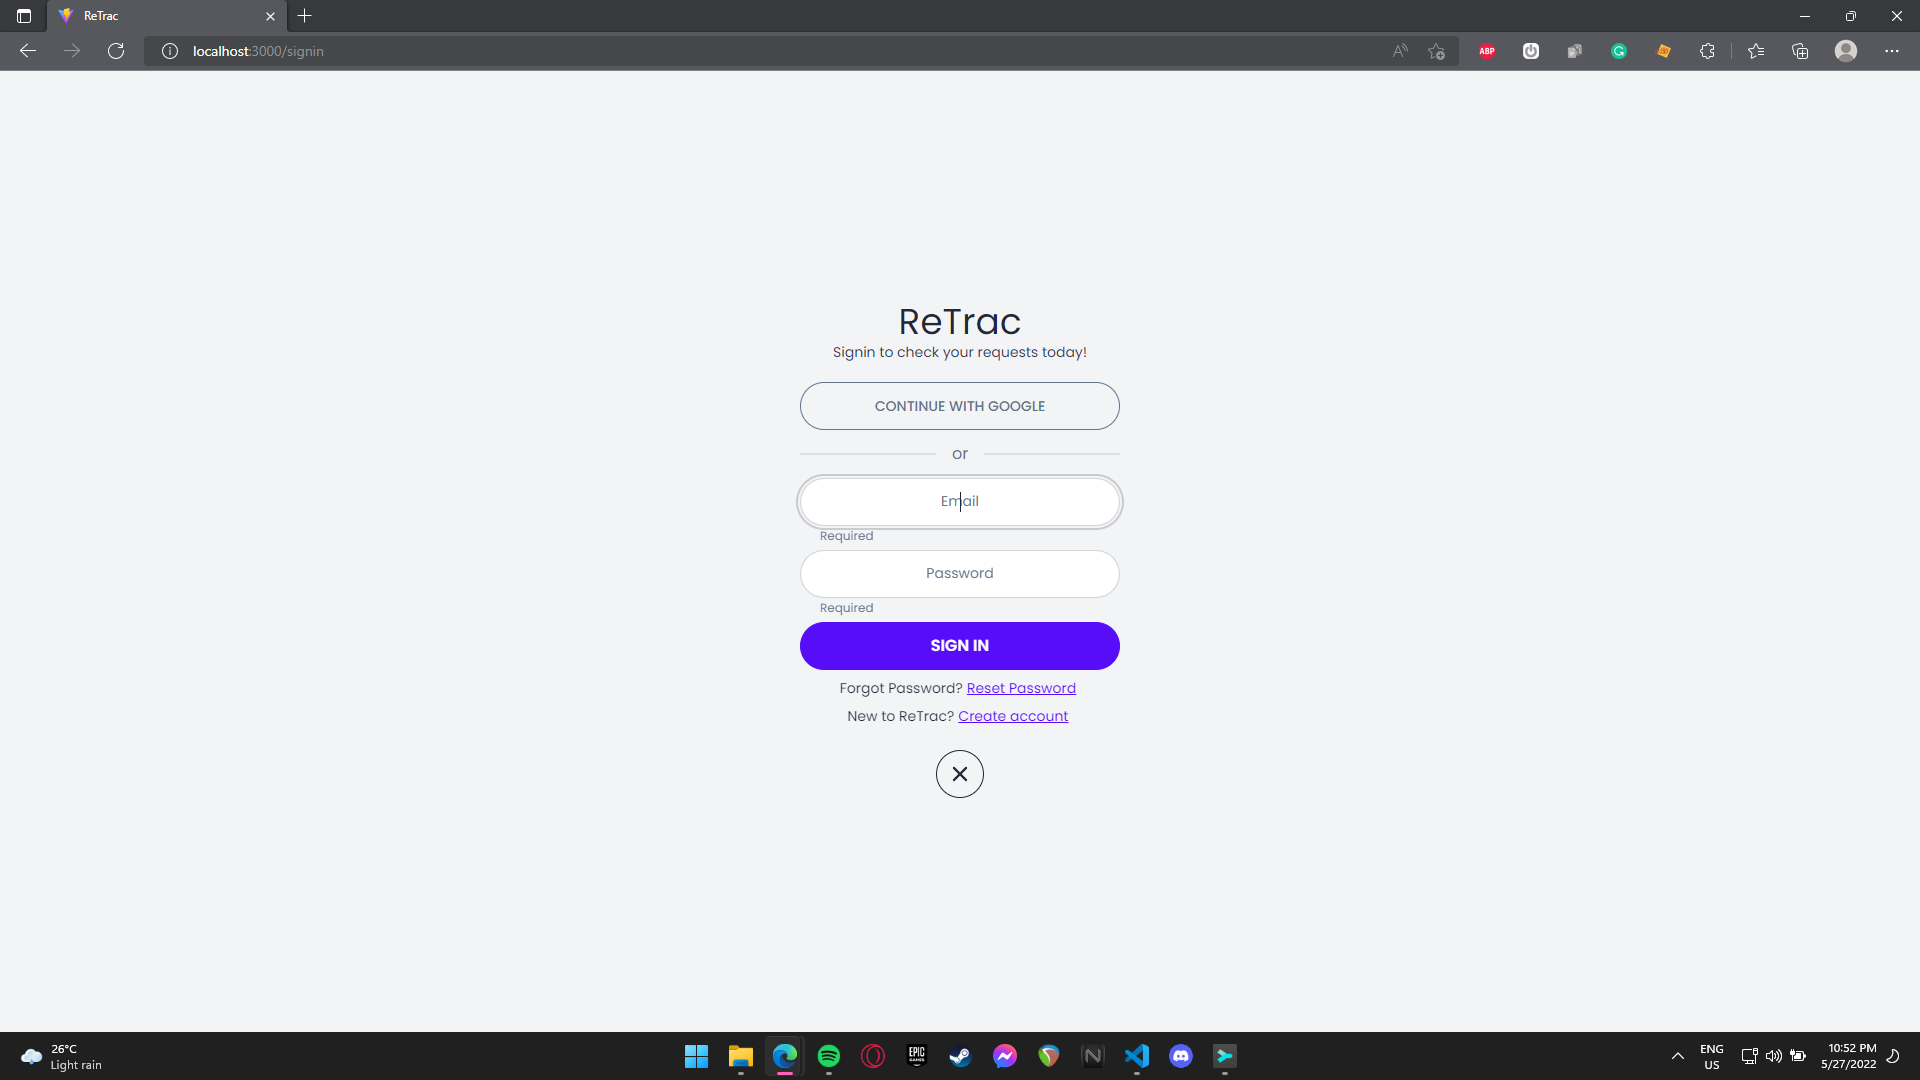
\includegraphics[width=0.9\columnwidth]{Signin.png}
            \caption{Sign in page}
            \label{fig:Signin}
        \end{minipage}\hfill
        \begin{minipage}[c]{0.5\linewidth}
            \centering
            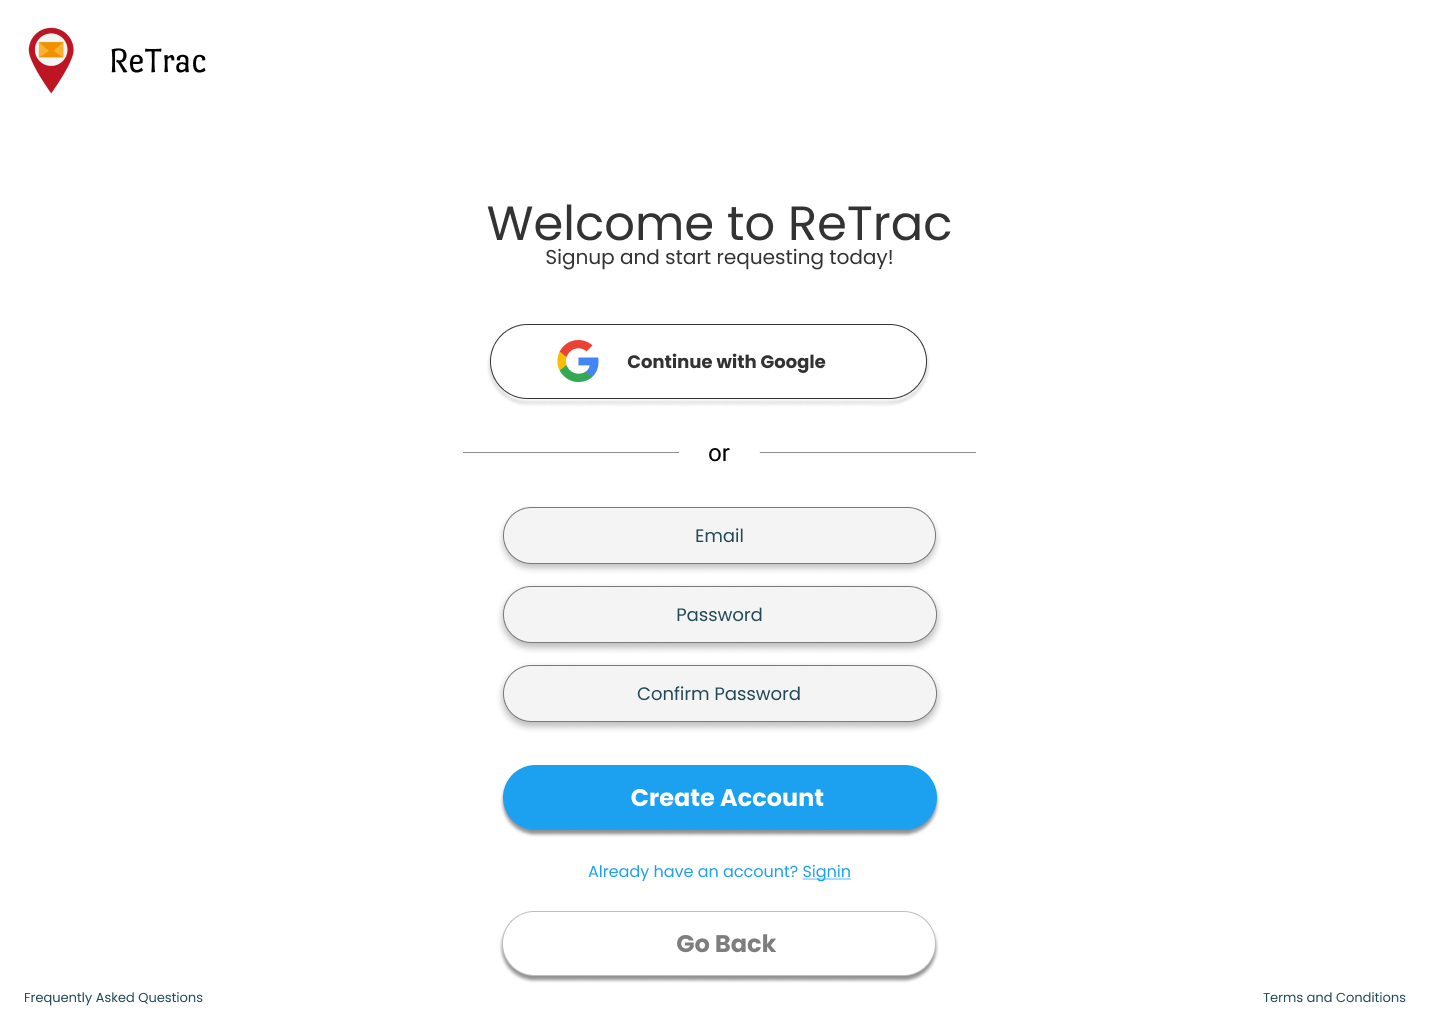
\includegraphics[width=0.9\columnwidth]{Signup.png}
            \caption{Sign up page}
            \label{fig:Signup}
        \end{minipage}
    \end{figure}

    \begin{figure}[h]
        \centering 
        \begin{minipage}[c]{0.5\linewidth}
            \centering
            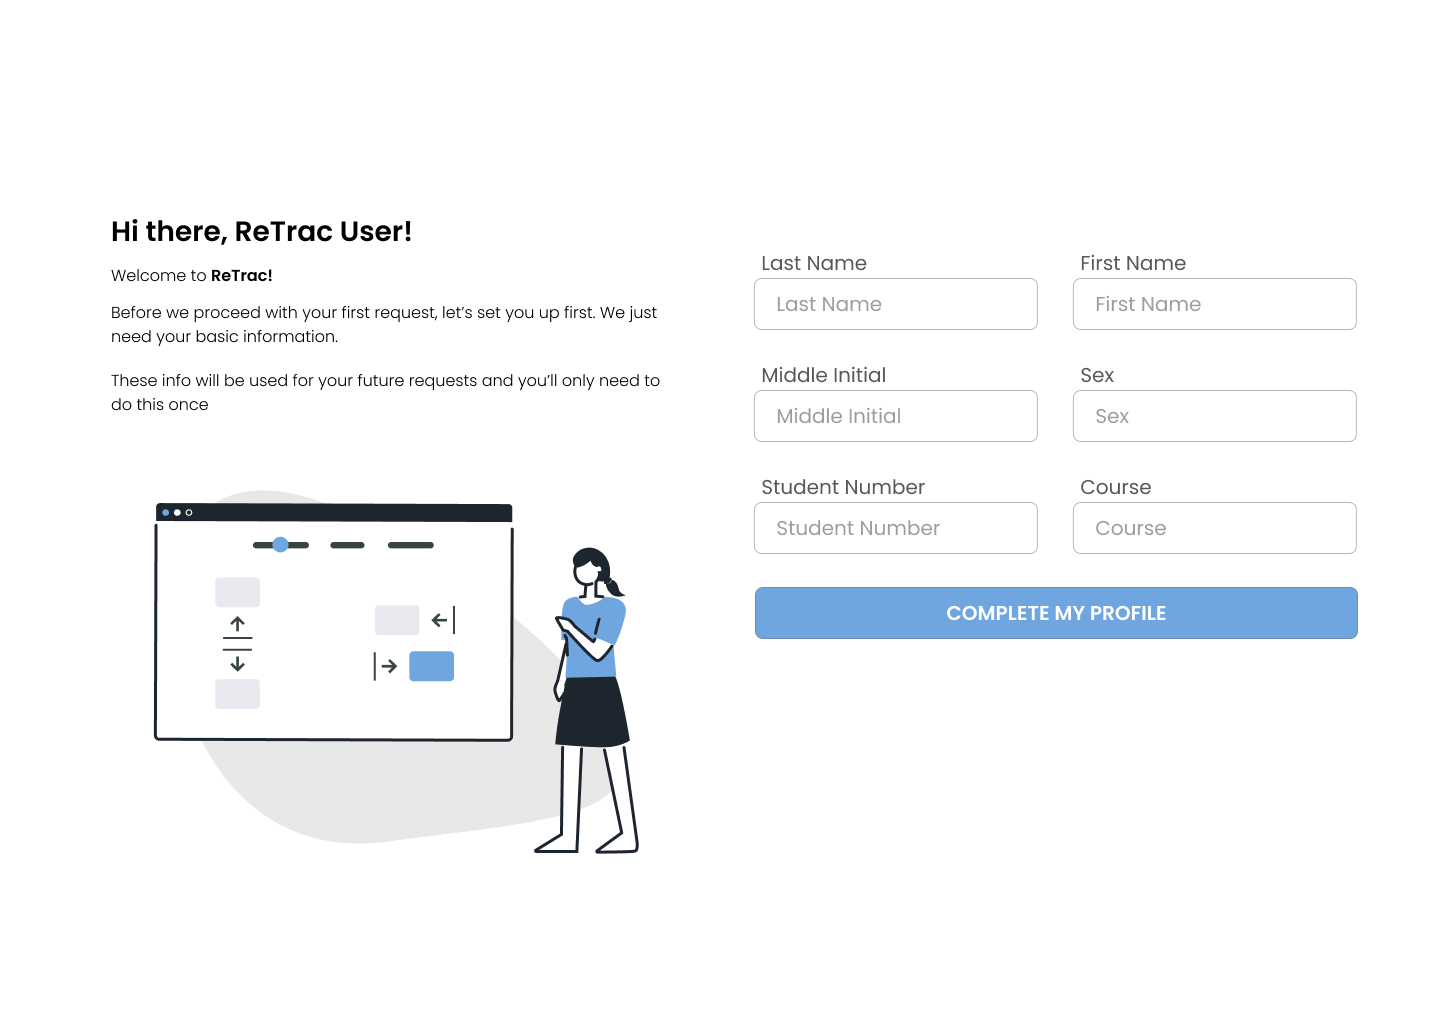
\includegraphics[width=0.9\columnwidth]{Welcome.png}
            \caption{Requestor's On-boarding page}
            \label{fig:Welcome}
        \end{minipage}
    \end{figure}

    \begin{figure}[h]
        \centering 
        \begin{minipage}[c]{0.5\linewidth}
            \centering
            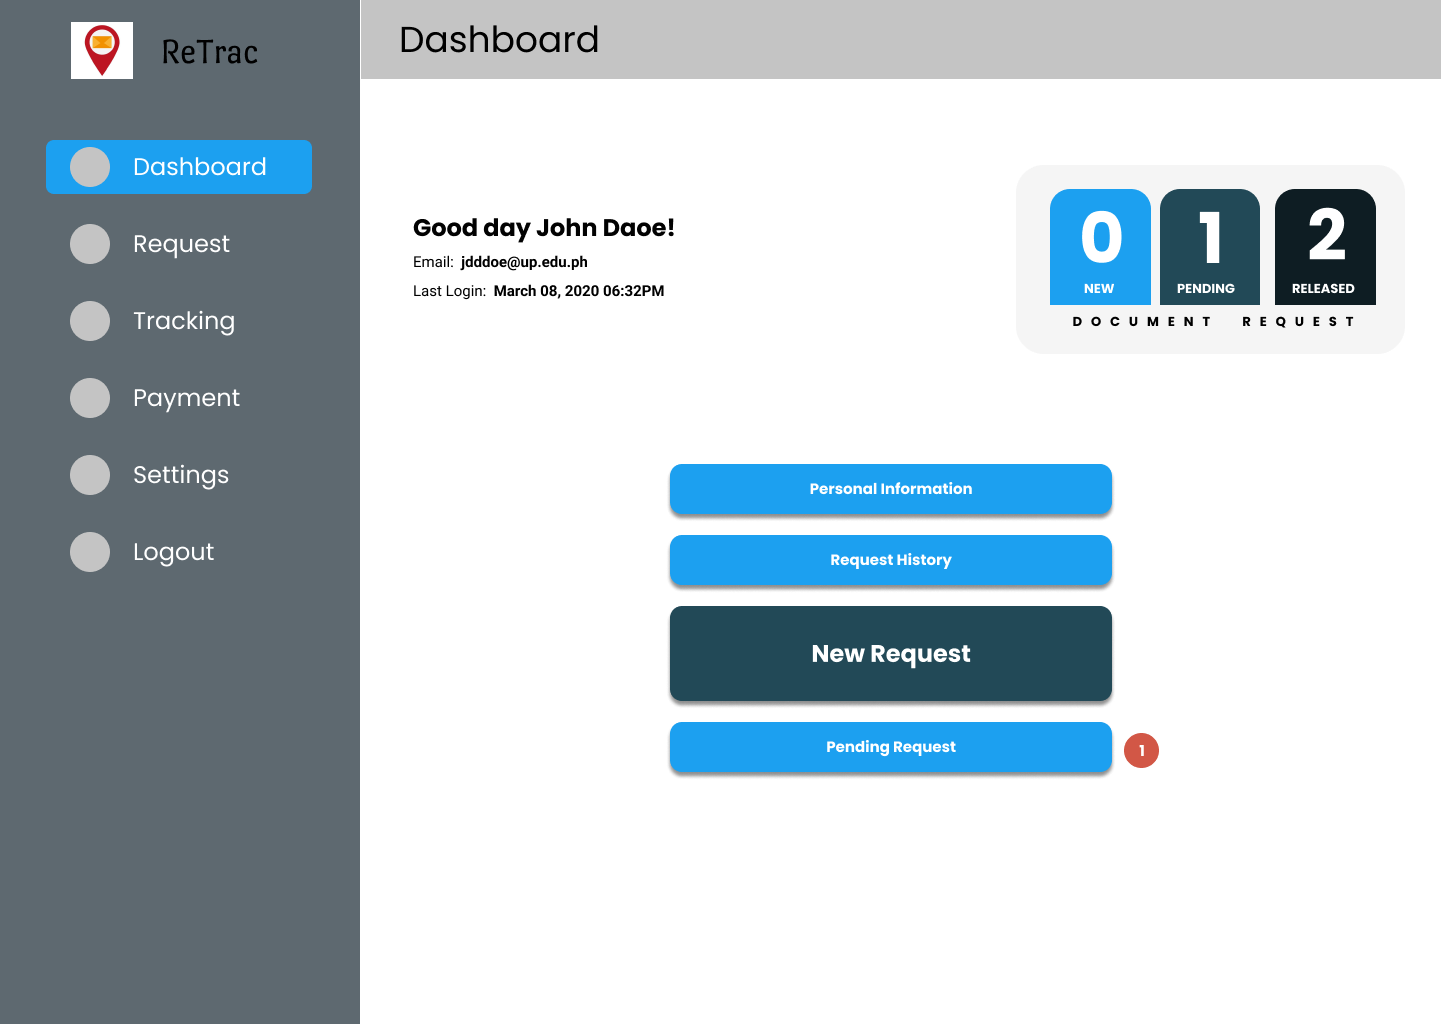
\includegraphics[width=0.9\columnwidth]{Dashboard.png}
            \caption{Requestor's Dashboard page}
            \label{fig:Dashboard}
        \end{minipage}
    \end{figure}


These features will let the user access their ReTrac profile in order to request documents, view pending and previous requests, and update their profile information. The user will need to sign up in order to utilize the system by providing their information. If the user is already registered, the sign-in page will collect their credentials and will redirect them to the dashboard where they will have a quick glance at their documents request in Figure 4.4 Dashboard. It is further divided into three status cards called “new”, “pending”, and “released”. By clicking on it, it will redirect to the tracking page with filtered results which will be discussed in the tracking section below.

\subsubsection{Request Page}

The Request Page is designed as a step-by-step form. It has four (4) steps, “Enter Details”, “Review Information”, “Payment”, and “Track Document”. This page features the requesting of possible documents from the CAS College Secretary with multiple documents at an instance.

    \begin{figure}[h]
        \centering 
        \begin{minipage}[c]{0.5\linewidth}
            \centering
            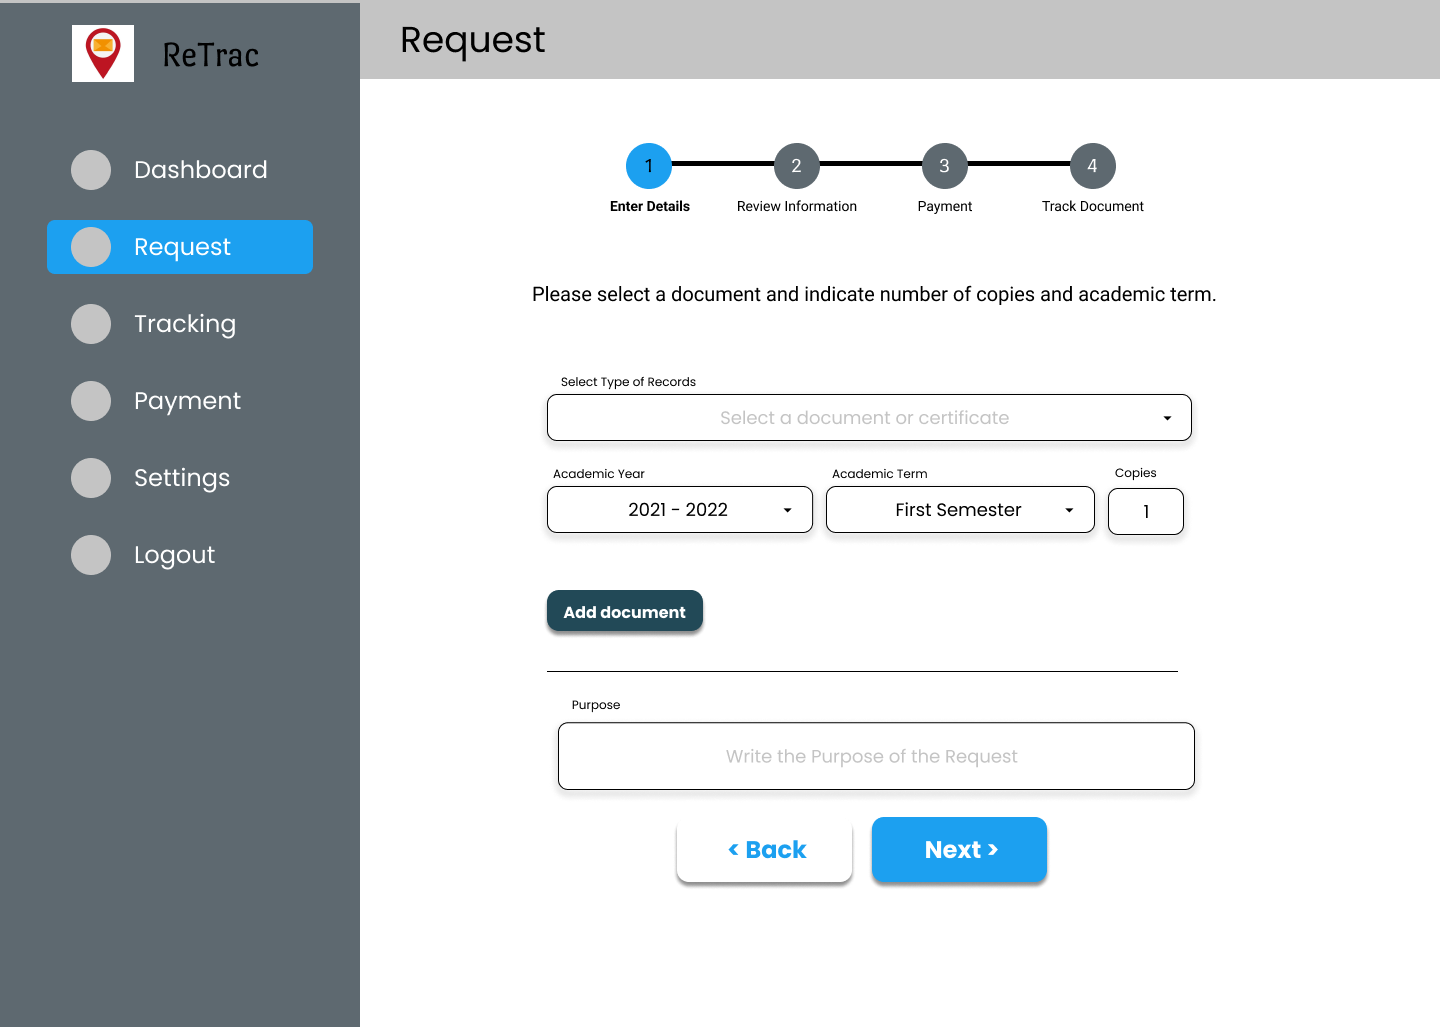
\includegraphics[width=0.9\columnwidth]{Request1.png}
            \caption{Fresh state of Request Page}
            \label{fig:Request1}
        \end{minipage}
    \end{figure}


    \begin{figure}[h]
        \centering 
        \begin{minipage}[c]{0.5\linewidth}
            \centering
            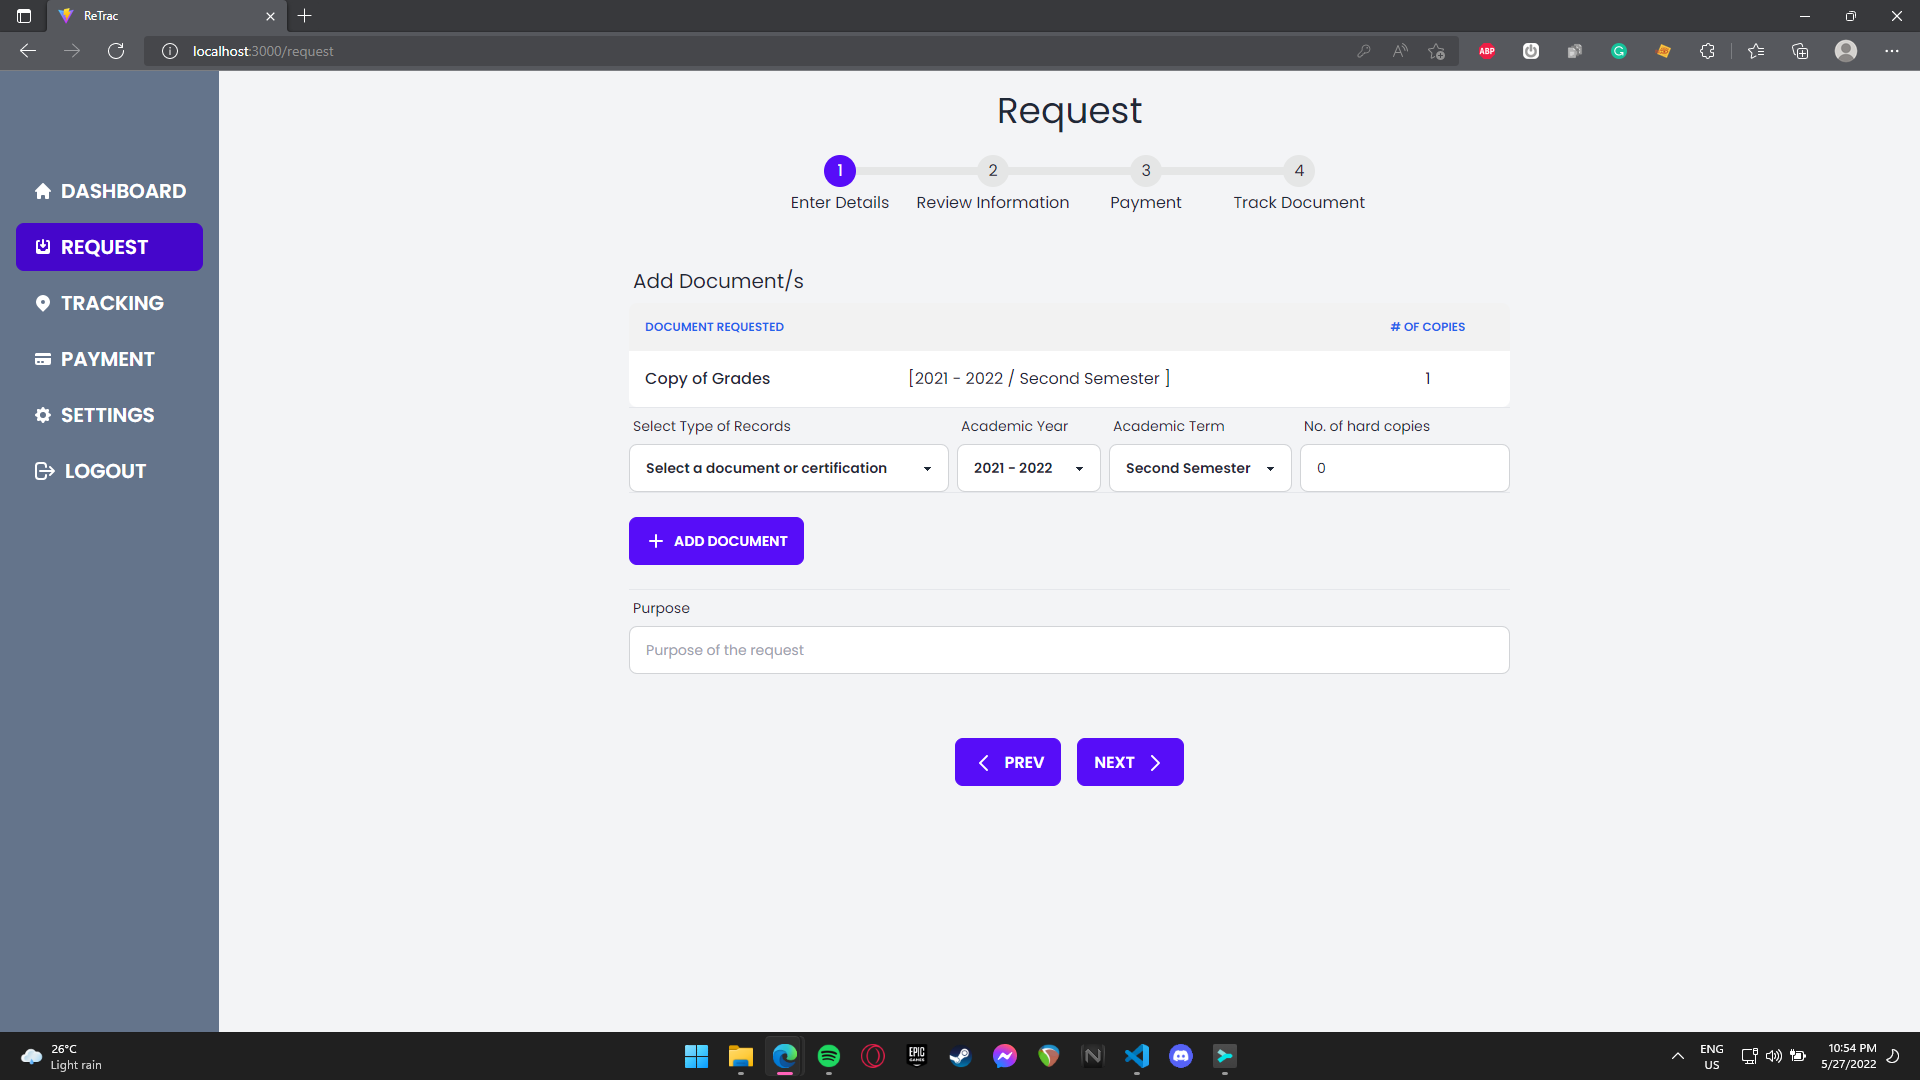
\includegraphics[width=0.9\columnwidth]{Request2.png}
            \caption{Documents added on the "Enter Details" step}
            \label{fig:Request2}
        \end{minipage}
    \end{figure}

When the user clicks on “New Request” from Figure 4.4 or on the sidebar, Figure 4.5 Fresh State Request Page will be displayed. The requestor is then greeted with this form which it will ask for the type of document, the academic year and term, number of copies, and purpose. 

Multiple documents may be requested per order or request. They can add different variants of documents using the “Add Document” button which will give them a cleared form with saved information of the previous documents at the top of the form as shown in Figure 4.6. Clicking the “Next” button will prompt the user to the Information Review page.

    \begin{figure}[h]
        \centering 
        \begin{minipage}[c]{0.5\linewidth}
            \centering
            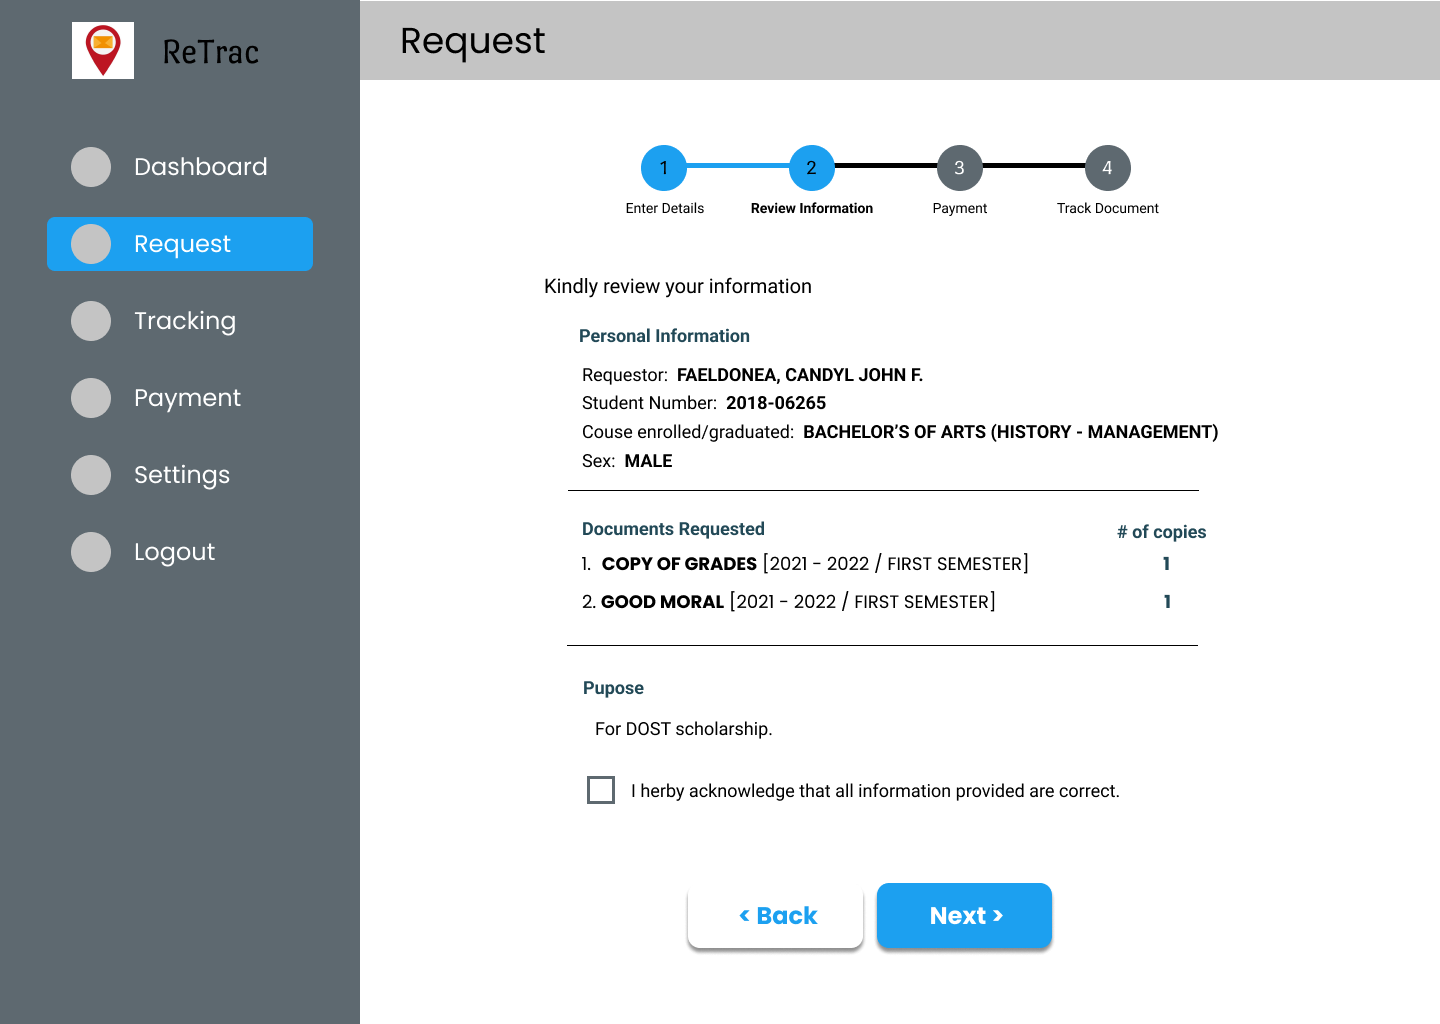
\includegraphics[width=0.9\columnwidth]{Request3.png}
            \caption{Information Review page}
            \label{fig:Request3}
        \end{minipage}\hfill
        \begin{minipage}[c]{0.5\linewidth}
            \centering
            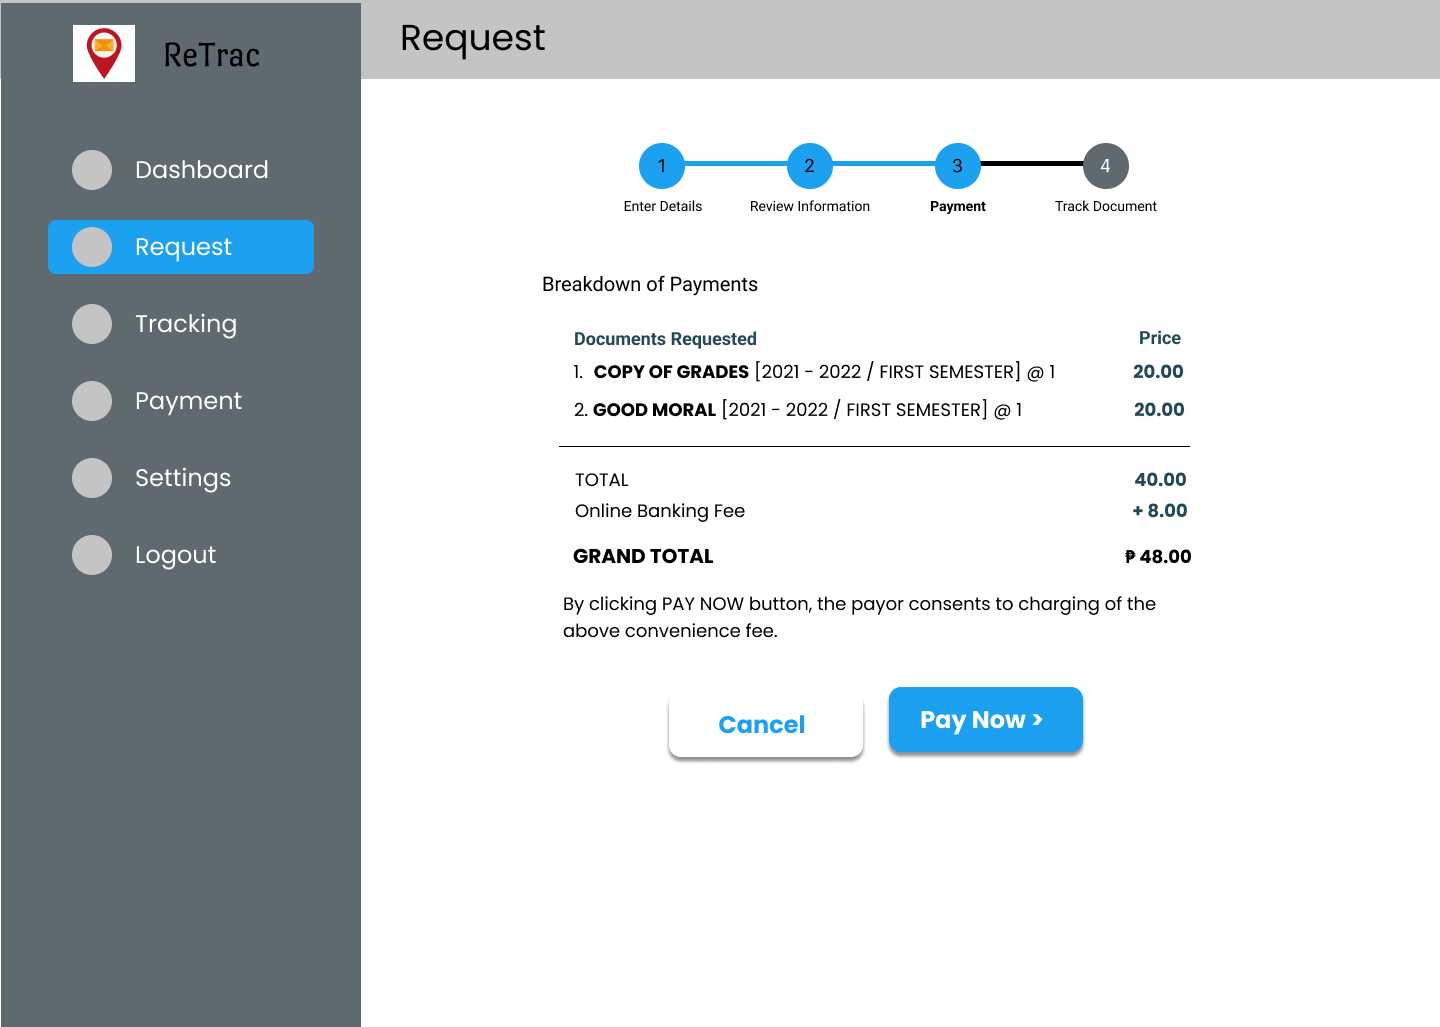
\includegraphics[width=0.9\columnwidth]{Request4.png}
            \caption{Payment Breakdown page}
            \label{fig:Request4}
        \end{minipage}
    \end{figure}

The Information Review Page will display a summary of documents requested as well the information of the requestor that will be processed by the CAS College Secretary. A safeguard checkbox is added so that the user will confirm that all the information provided is correct to the best of their ability. Figure 4.8 shows the breakdown of payments based on the documents requested. The user can then pay using the QR code provided by the Cash Office in Figure 4.9.

    \begin{figure}[h]
        \centering 
        \begin{minipage}[c]{0.5\linewidth}
            \centering
            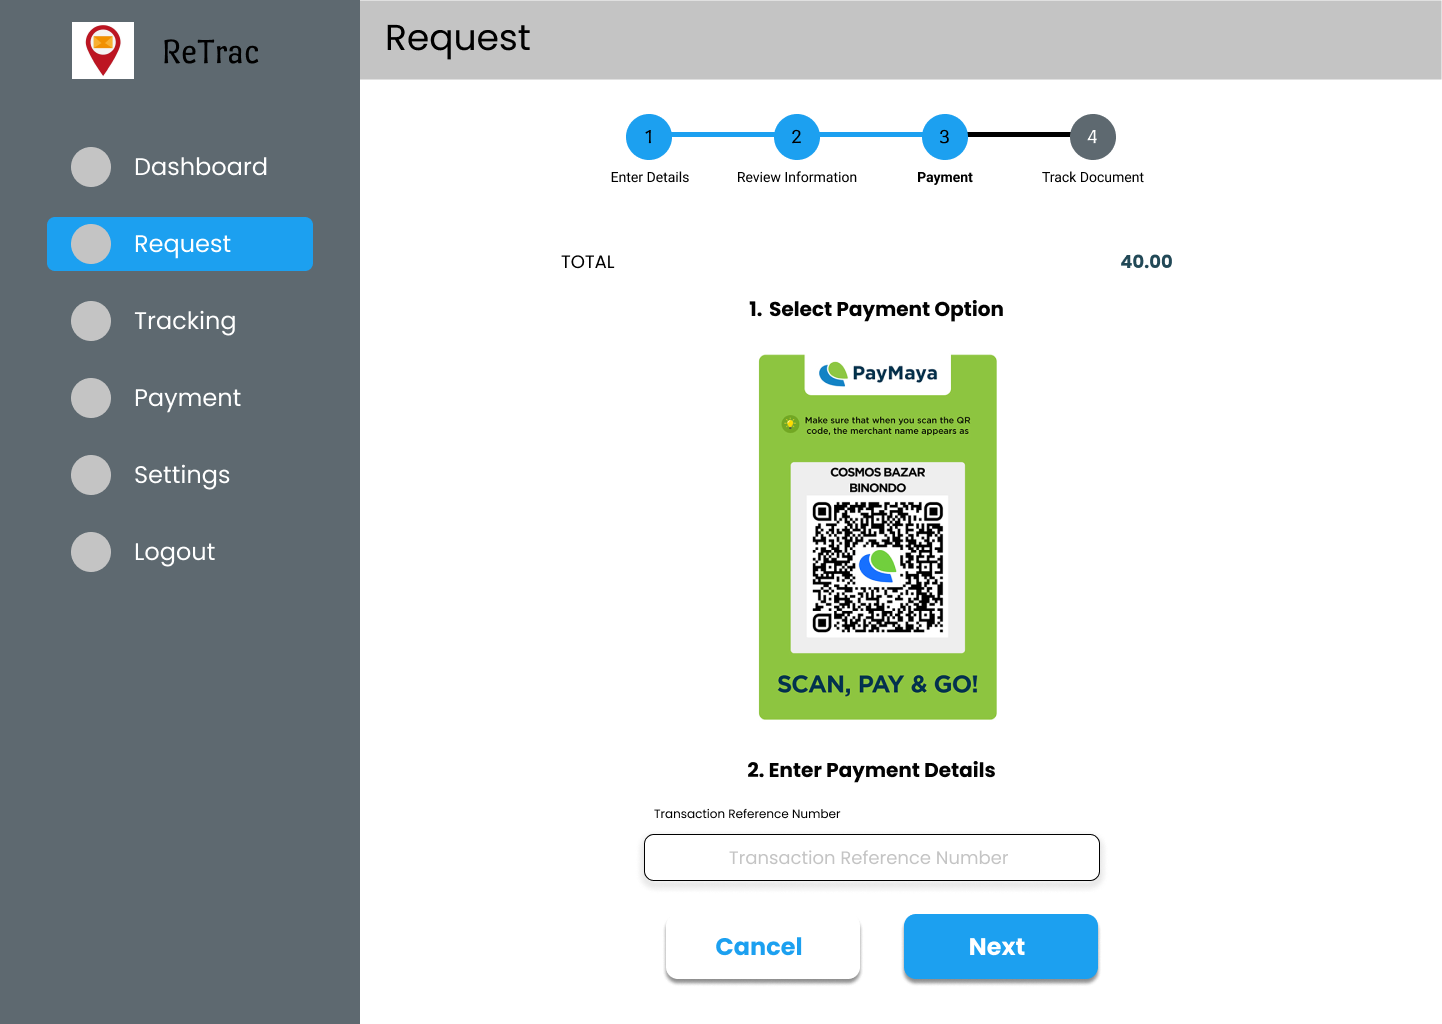
\includegraphics[width=0.9\columnwidth]{Request5.png}
            \caption{Payment QR code page}
            \label{fig:Request5}
        \end{minipage}\hfill
        \begin{minipage}[c]{0.5\linewidth}
            \centering
            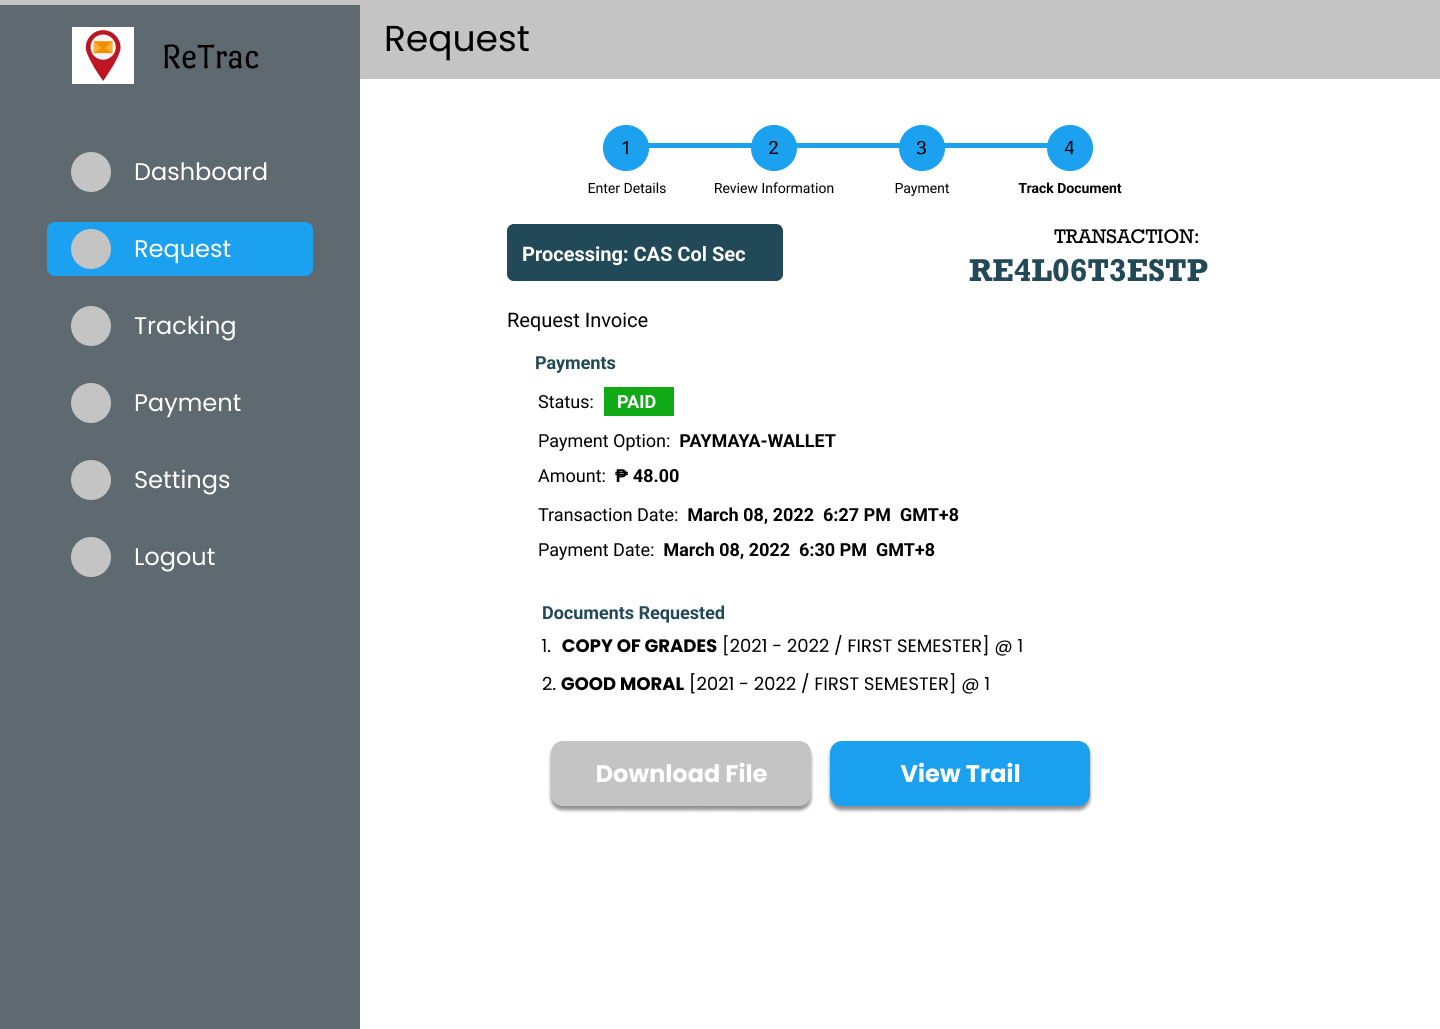
\includegraphics[width=0.9\columnwidth]{Request6.png}
            \caption{Invoice Page}
            \label{fig:Request6}
        \end{minipage}
    \end{figure}

The Payment QR page is under the payment step where the requester will be scanning the QR code of an online payment provider. The user then enters the transaction reference number manually for verification by the Cash Office which will be discussed in the later section. After entering the number, it will display the initial tracking page and transaction information which includes the request transaction code, transaction dates, and documents requested. The requestor has options to either cancel the entire transaction or view the trail of requests, the latter will redirect them to the tracking page feature.

\subsubsection{Tracking Page}

The Tracking Page will help the requester track the documents requested into four (4) categories: All, Paid, Processing, and Completed.  The requester on the feature will be able to see the request trail, download documents, confirmed receiving of documents, and get status updates.

    \begin{figure}[h]
        \centering 
        \begin{minipage}[c]{0.5\linewidth}
            \centering
            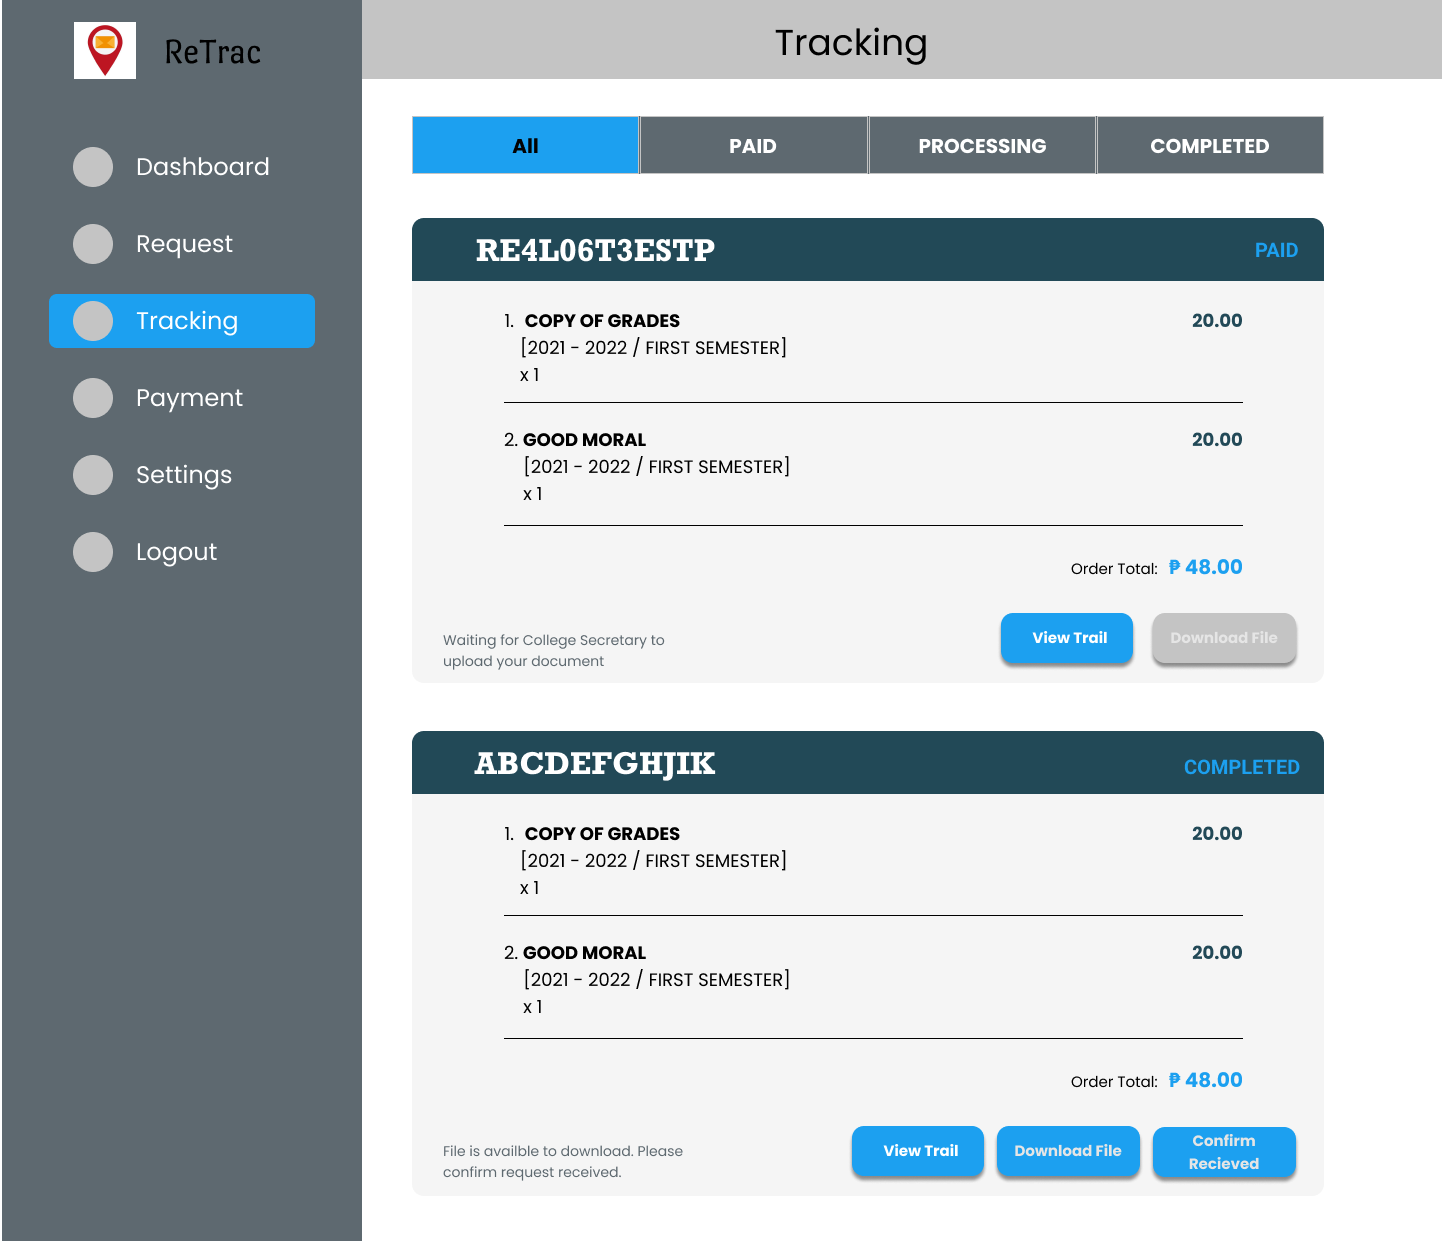
\includegraphics[width=0.9\columnwidth]{Tracking1.png}
            \caption{Tracking Main page}
            \label{fig:Tracking1}
        \end{minipage}\hfill
        \begin{minipage}[c]{0.5\linewidth}
            \centering
            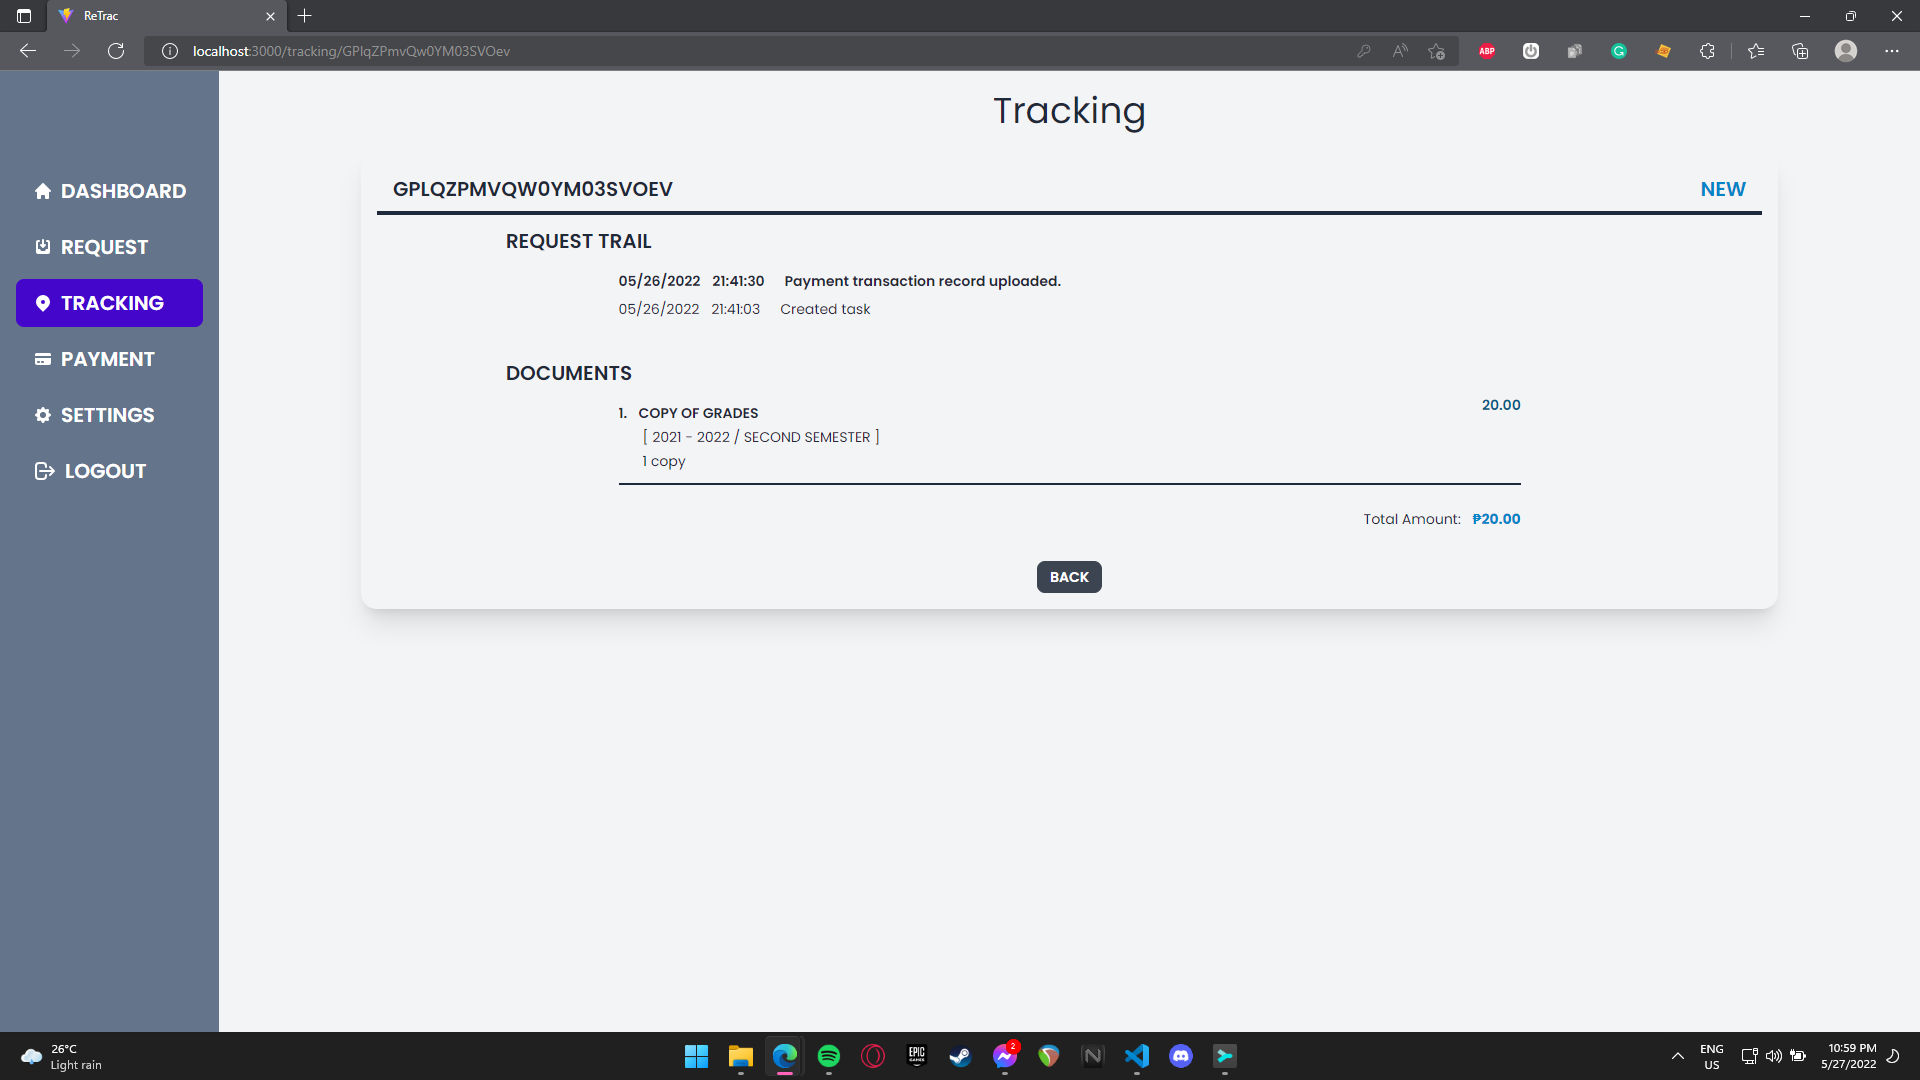
\includegraphics[width=0.9\columnwidth]{Tracking2.png}
            \caption{Tracking - Request Trail page}
            \label{fig:Tracking2}
        \end{minipage}
    \end{figure}

The Tracking Main Page shown in Figure 4.12 shows all paid requests made by the user. The user can further filter out the request by “Paid”, “ Processing”, and “Completed”. In the case where the status of the document is “Paid” or “Processing”, the requester will only be able to see the request trail. When the status is set to “completed”, the requester can access the request trail, download the file immediately, and/or mark the request as received. On Figure 4.12, this shows the offices where the paper is currently being processed. It also displays the date stamps of the request milestones. In the case the College Secretary uploads the file, an email notifcation will be sent to the requestor, and the user will have a week to confirm receipt of the documents before it is automatically marked as received.

\subsection{UPV Cash Office View}

This section will discuss the different features of the UPV Cash Office View which will be used by the staff of the UPV Cash Office.

\subsubsection{Dashboard}

The Cash Office will have the same Sign up page as the requestor, however, the system will redirect them to their own privileged dashboard as shown in Figure 4.13.
    \begin{figure}[h]
        \centering 
        \begin{minipage}[c]{0.5\linewidth}
            \centering
            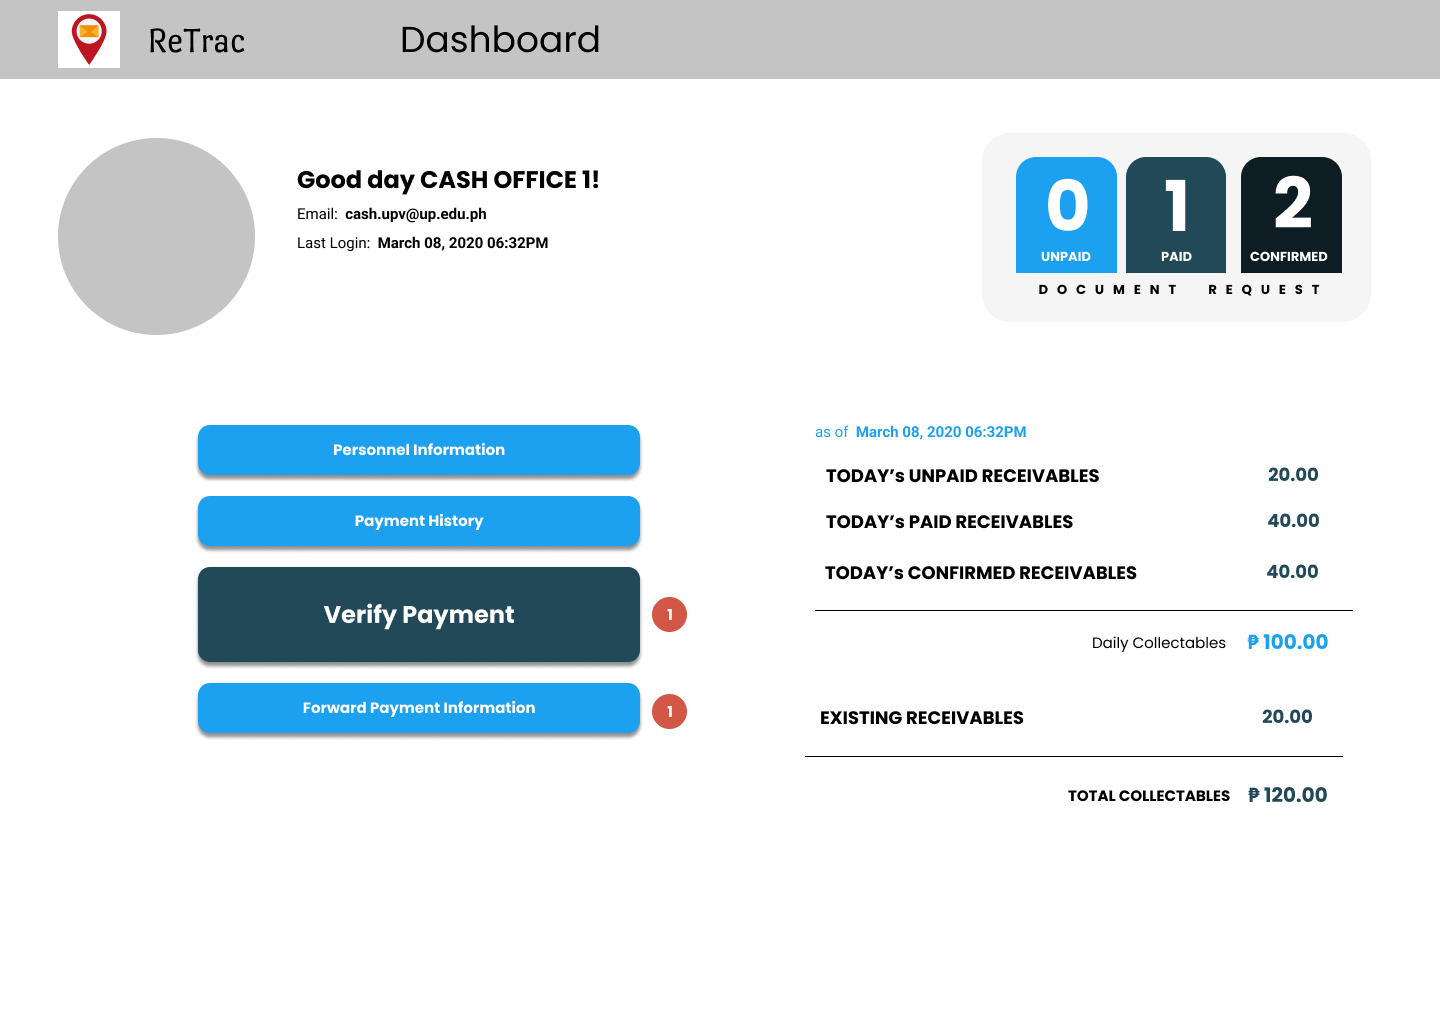
\includegraphics[width=0.9\columnwidth]{CO_Dashboard.png}
            \caption{Cash Office Dashboard page}
            \label{fig:CO_Dashboard}
        \end{minipage}
    \end{figure}

The dashboard will show the credentials of the cash office, and the last login timestamp of the office. The upper-ride corner holds statistics of the receivable payments in the form of “Unpaid”, “Paid”, and “Confirmed”. The page\textsc{\char13}s center houses buttons that will redirect the office into accessing their profile, payment history, payment verification, and payment information forwarding. All of these will be discussed further below.

\subsubsection{All Payments View}

    \begin{figure}[h]
        \centering 
        \begin{minipage}[c]{0.5\linewidth}
            \centering
            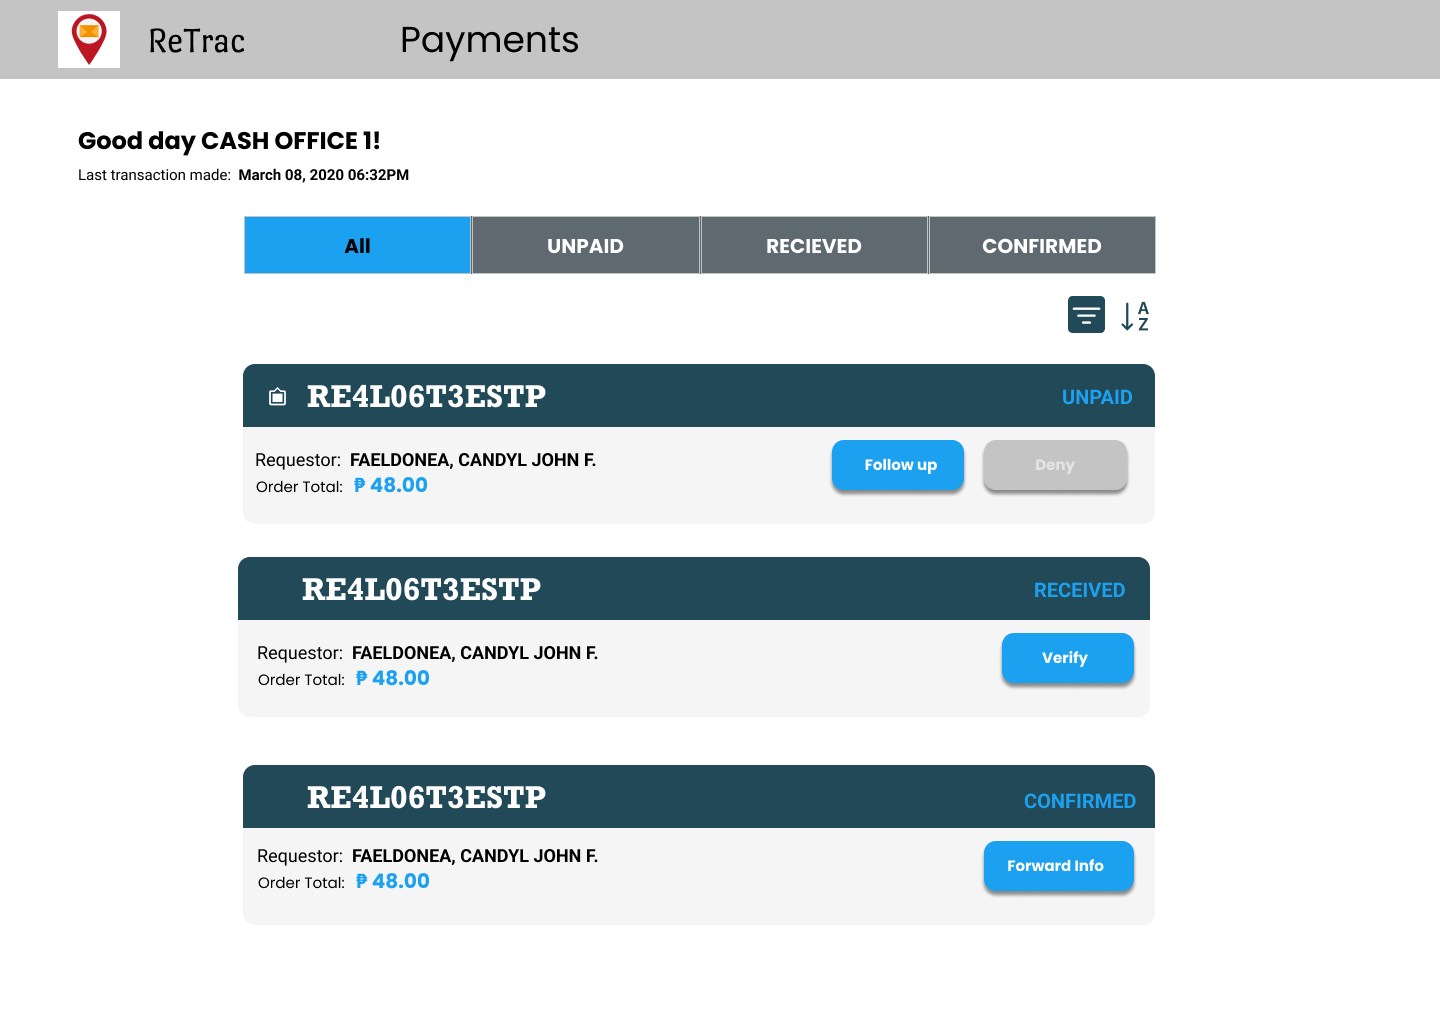
\includegraphics[width=0.9\columnwidth]{CO_Payments.png}
            \caption{List of Active Payment Page}
            \label{fig:CO_Payments}
        \end{minipage}
    \end{figure}

This page will show all the active payments that are not forwarded to the College Secretary. This further classifies the payments into Unpaid, Received, and Confirmed. For payments with the status “unpaid”, the cash office may follow up or deny the request. For “received”, they verify the payment made by the requestor. Lastly, when the status is “confirmed”  they have the option to forward information to the college secretary, then the record will only be visible on the “Payment History Page”.

\subsubsection{Verification and Original Receipt Forwarding}

This page will display the partial payment details entered by the requestor in Figure 4.9. The office will need to enter the reference number they received on their end and when verified will redirect them to the official receipt uploading page in Figure 4.16 where they will be entering the official receipt transaction number and the file itself for the record of the college secretary. This will then archive the transaction.

\begin{figure}[h]
    \centering 
    \begin{minipage}[c]{0.5\linewidth}
        \centering
        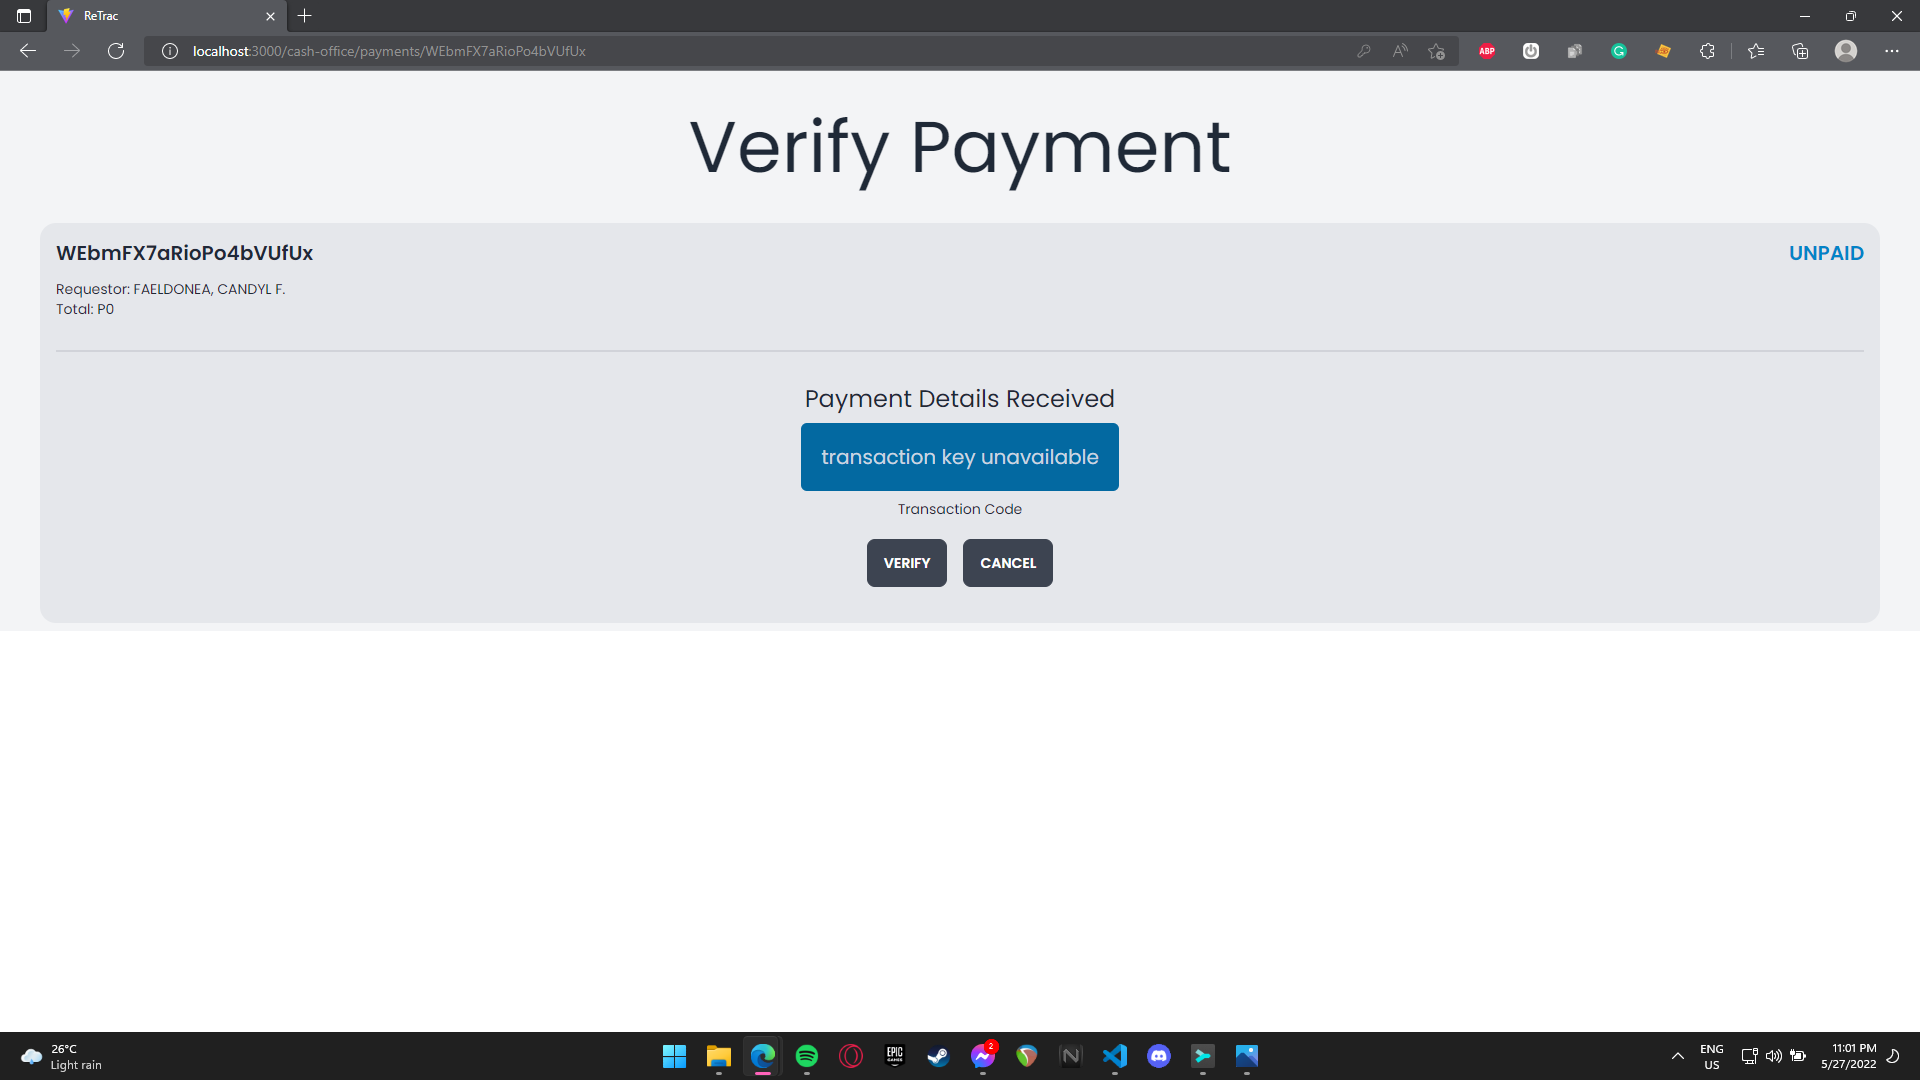
\includegraphics[width=0.9\columnwidth]{CO_VerifyPayments.png}
        \caption{Payment Verification Page}
        \label{fig:CO_VerifyPayments}
    \end{minipage}
\end{figure}

\begin{figure}[h]
    \centering 
    \begin{minipage}[c]{0.5\linewidth}
        \centering
        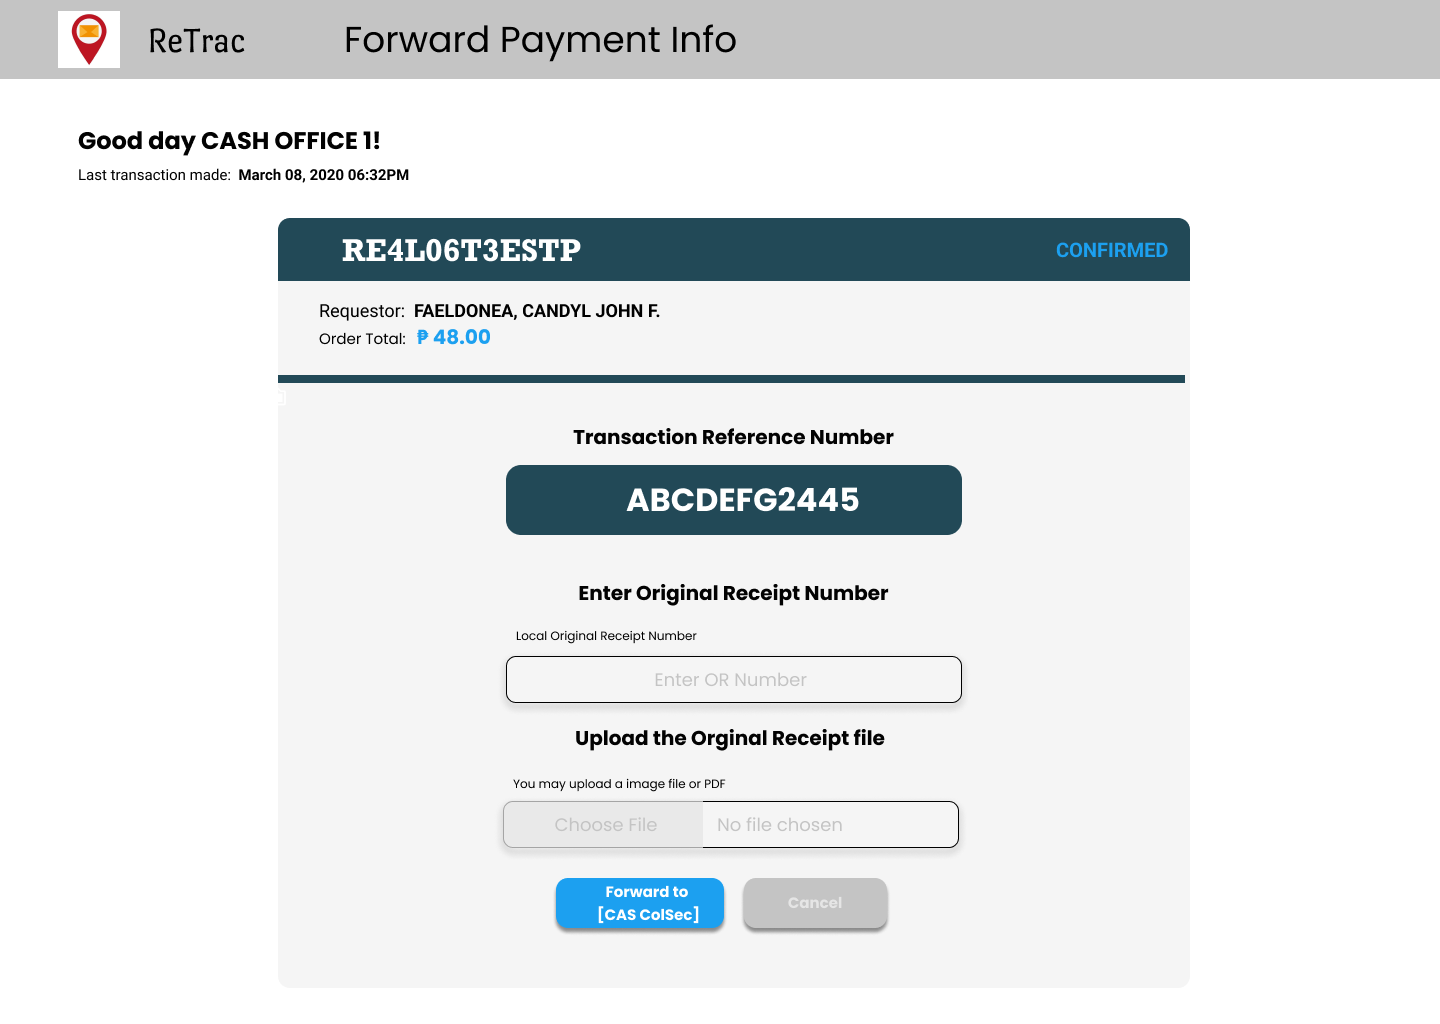
\includegraphics[width=0.9\columnwidth]{CO_ForwardPayment1.png}
        \caption{OR file uploading page}
        \label{fig:CO_ForwardPayment1}
    \end{minipage}\hfill
    \begin{minipage}[c]{0.5\linewidth}
        \centering
        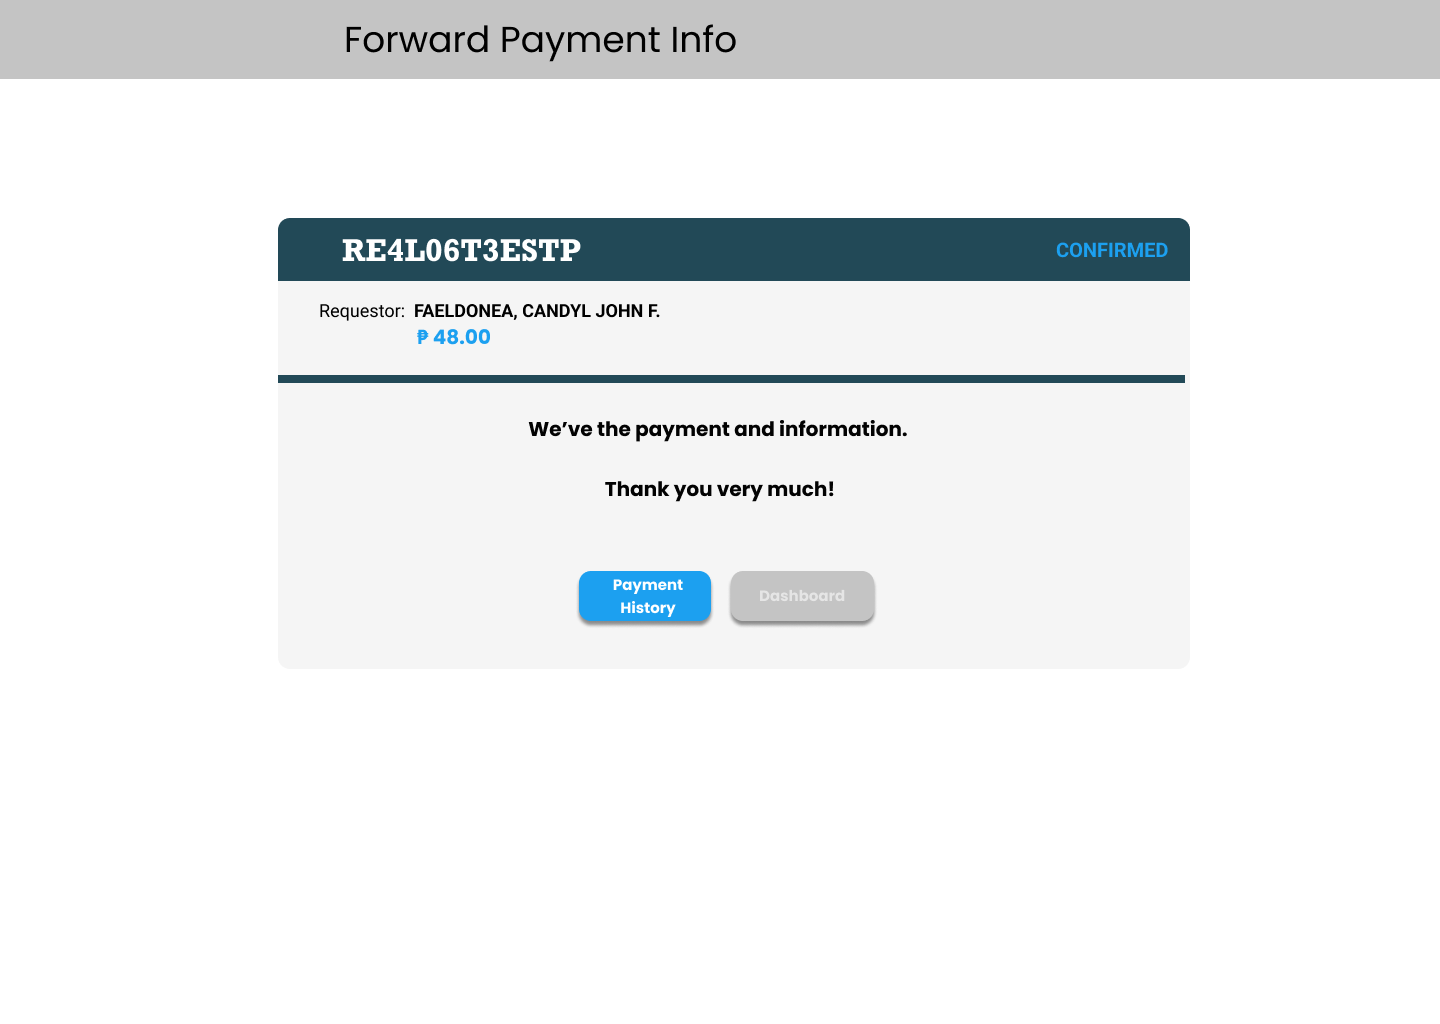
\includegraphics[width=0.9\columnwidth]{CO_ForwardPayment2.png}
        \caption{Payment and OR Confirmation notice}
        \label{fig:CO_ForwardPayment2}
    \end{minipage}
\end{figure}

In case the payment code provided by the user doesn\textsc{\char13}t match the code received by the office, they can mark the transaction as invalid.

\subsubsection{Payment History}

This page will give the cash office payment reports as well as monitoring of all the transactions that go in and out of their office.

\begin{figure}[h]
    \centering 
    \begin{minipage}[c]{0.5\linewidth}
        \centering
        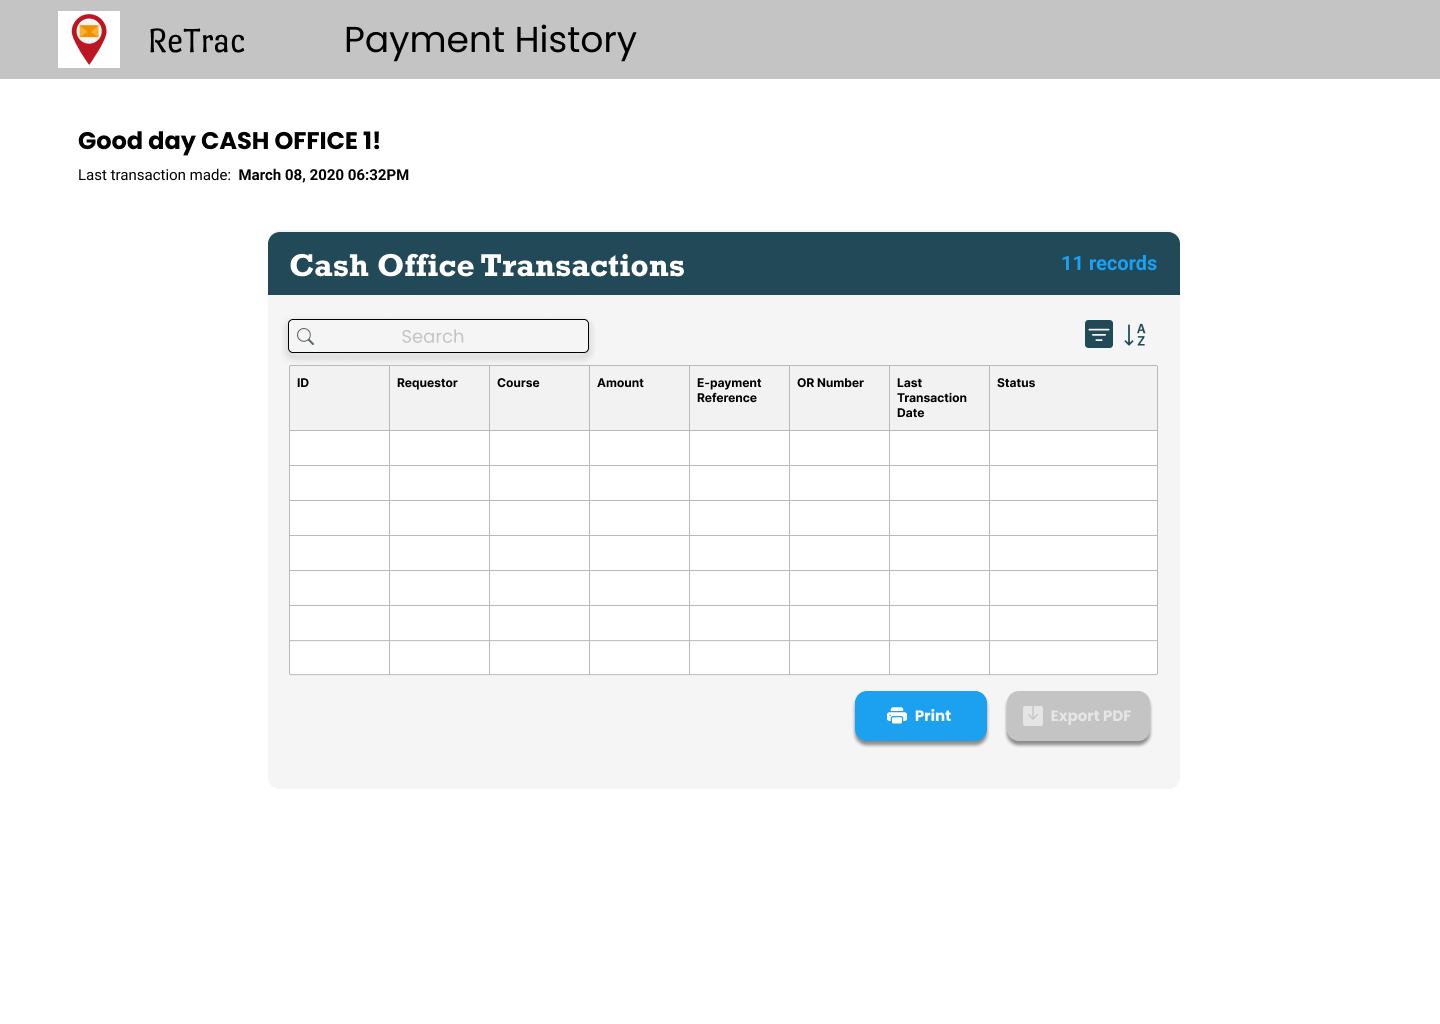
\includegraphics[width=0.9\columnwidth]{CO_PaymentHistory.png}
        \caption{Payment History Code}
        \label{fig:CO_PaymentHistory}
    \end{minipage}
\end{figure}

A read-only  Request History page will feature a table report where the office can either print or export the tables as a PDF file. It has sorting and search features. This will give the office a quick glance at the transactions including those forwarded to the college secretary.


\subsection{CAS College of the College Secretary View}

This section will discuss the different features of the CAS Office of the College Secretary View which will be used by the staff of the CAS Office of the College Secretary.



\subsubsection{Dashboard}
The College Secretary will have the same Sign up page as the requestor, however, the system will redirect them to their own privileged dashboard as shown in Figure 4.19. 

    \begin{figure}[h]
        \centering 
        \begin{minipage}[c]{0.5\linewidth}
            \centering
            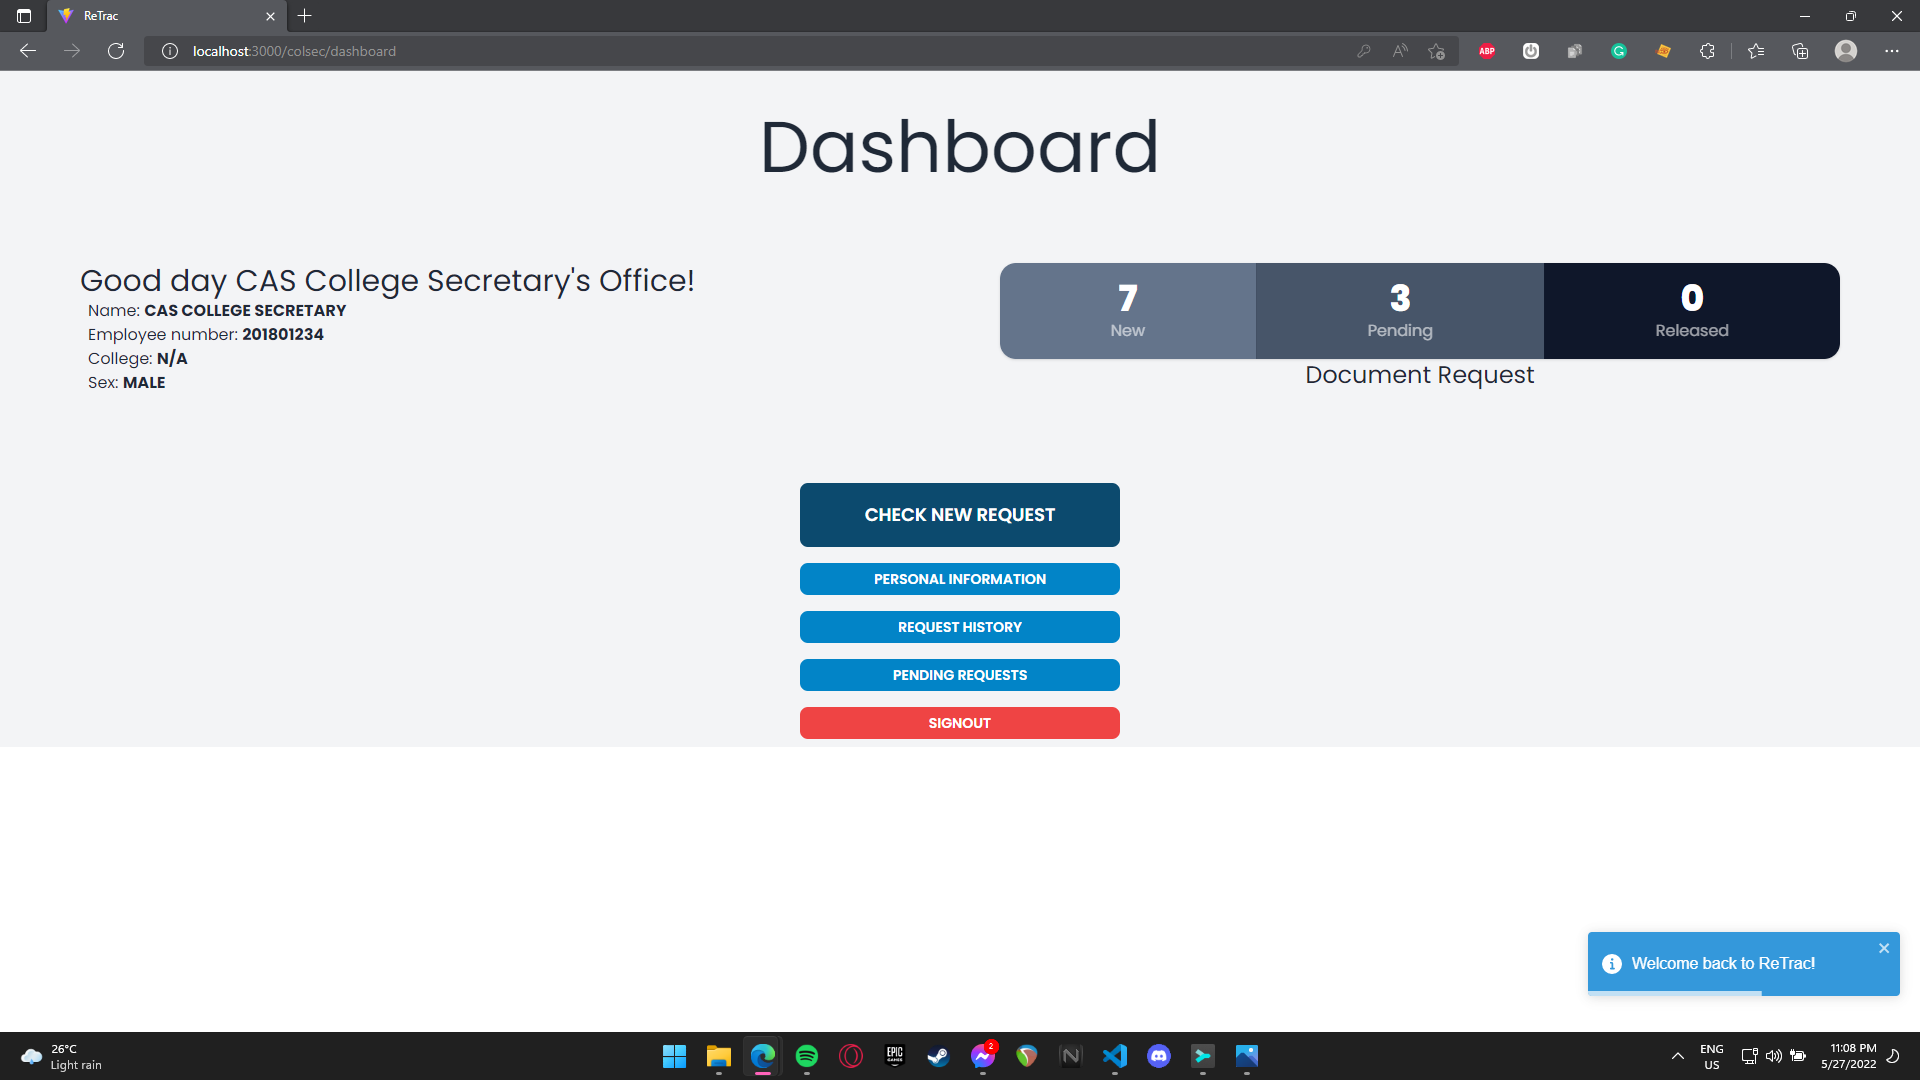
\includegraphics[width=0.9\columnwidth]{CS_Dashboard.png}
            \caption{CAS College Secretary Dashboard}
            \label{fig:CS_Dashboard}
        \end{minipage}
    \end{figure}

This dashboard will show the credentials of the college secretary, and the last login timestamp of the office. This will provide security information for the office. On the right-hand side, resides the notification statistics of the document requested in the form of “New”, “Pending”, and “Released” this mirrors the notification on the view of the requestor. The middle portion of the page contains buttons that will redirect the office into accessing their profile, history of request, new request, and pending request. This will be further discussed below.

\subsubsection{All Requests View}

\begin{figure}[h]
    \centering 
    \begin{minipage}[c]{0.5\linewidth}
        \centering
        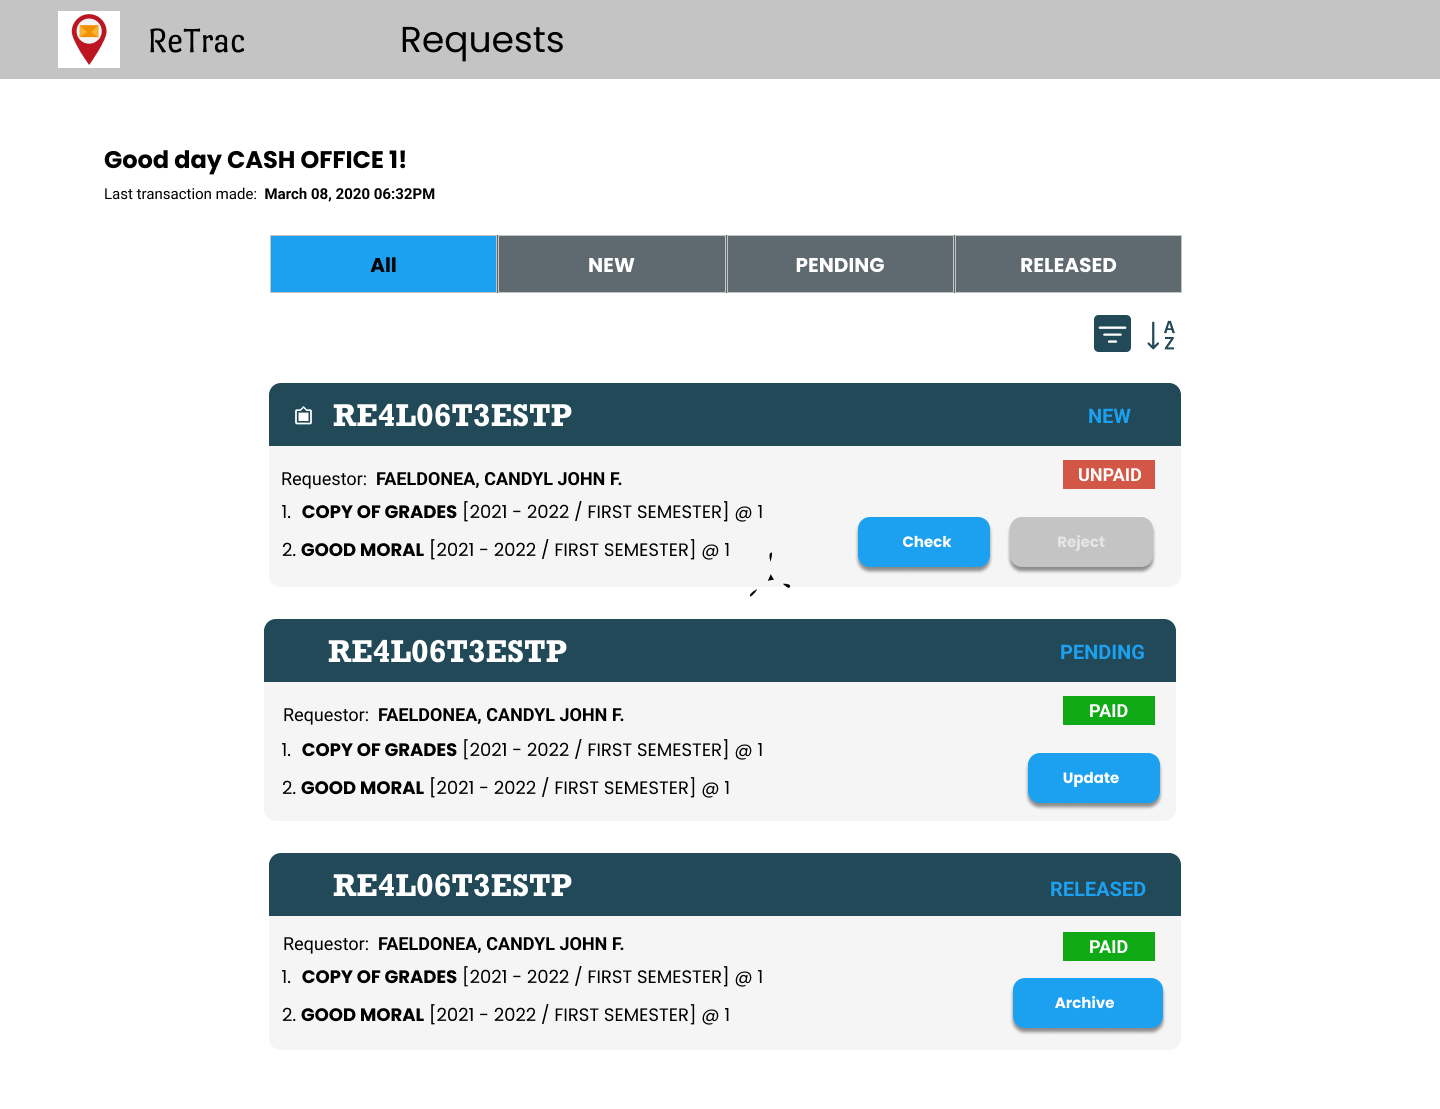
\includegraphics[width=0.9\columnwidth]{CS_Request1.png}
        \caption{List of Active Request Page}
        \label{fig:CS_Request1}
    \end{minipage}
\end{figure}

This page will show all the active requests that are not archived by the office. This is further classified into New, Pending, and Release. For requests with the status “new”, the college secretary may check or reject the request. For “pending”, they can provide updates specifically on the request trail or upload the file to be released. Lastly, when the status is “completed”  they have the option to archive the file which will only be visible on the “Request History Page”.

\subsubsection{Specific Request Check, Update, and Upload View}

This page features a specific request view where the office can check the information of the request including the requestor, the documents needed, and the payment status.


\begin{figure}[h]
    \centering 
    \begin{minipage}[c]{0.5\linewidth}
        \centering
        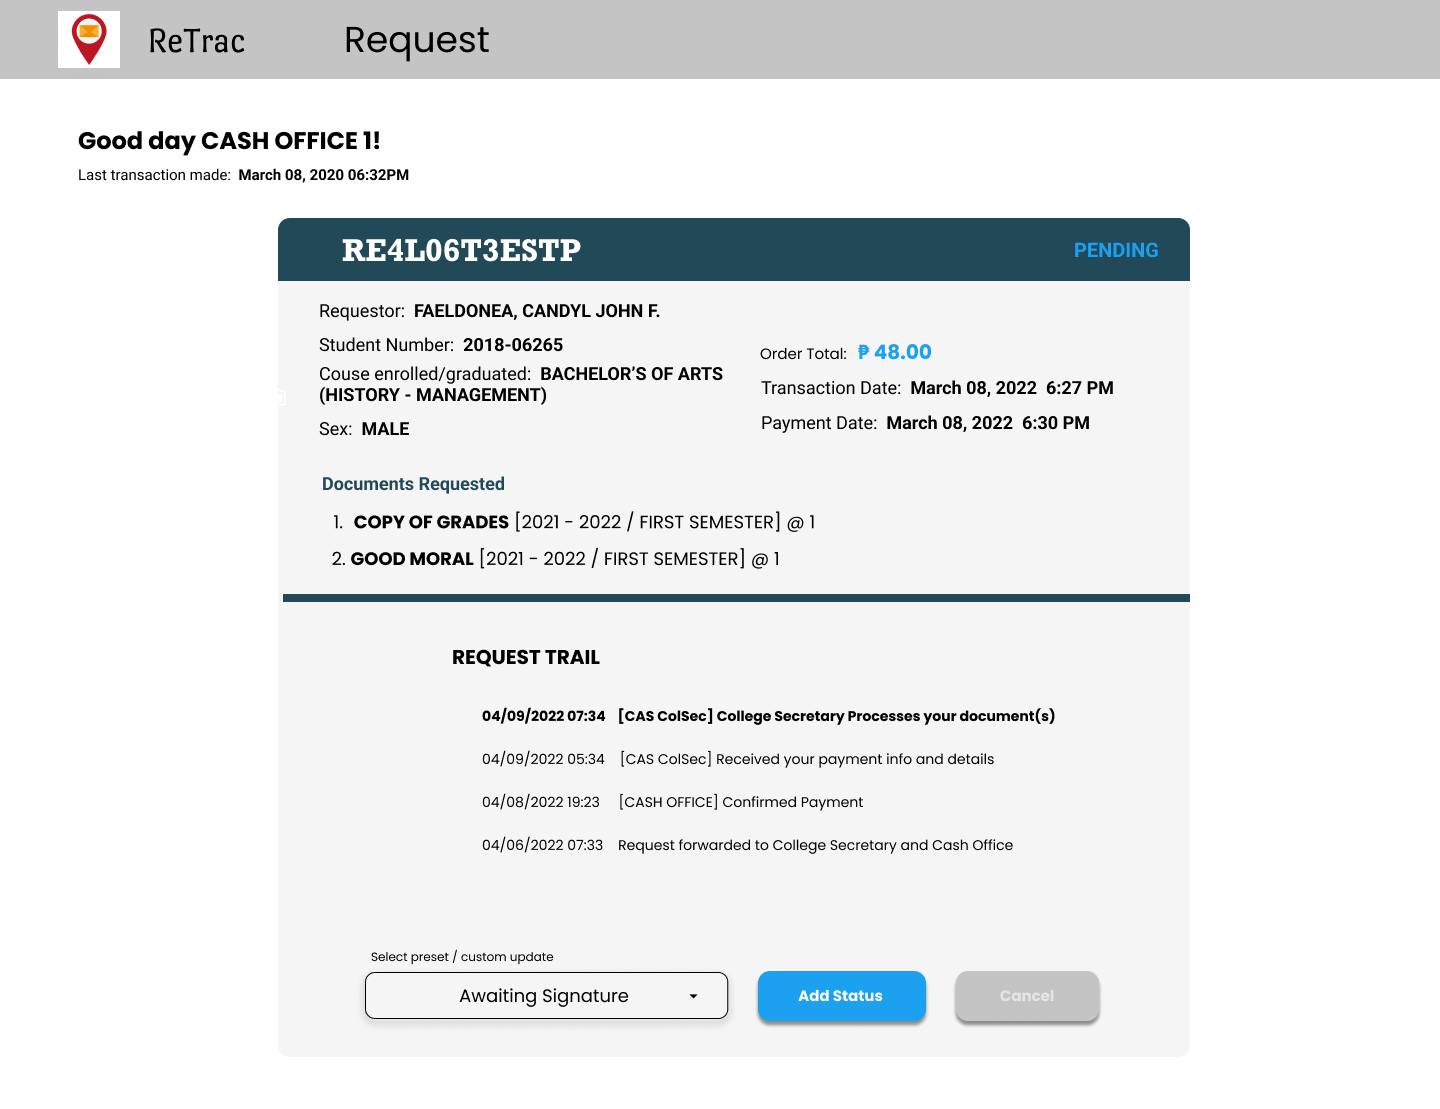
\includegraphics[width=0.9\columnwidth]{CS_Request2.png}
        \caption{Check and Status Update page}
        \label{fig:CS_Request2}
    \end{minipage}\hfill
    \begin{minipage}[c]{0.5\linewidth}
        \centering
        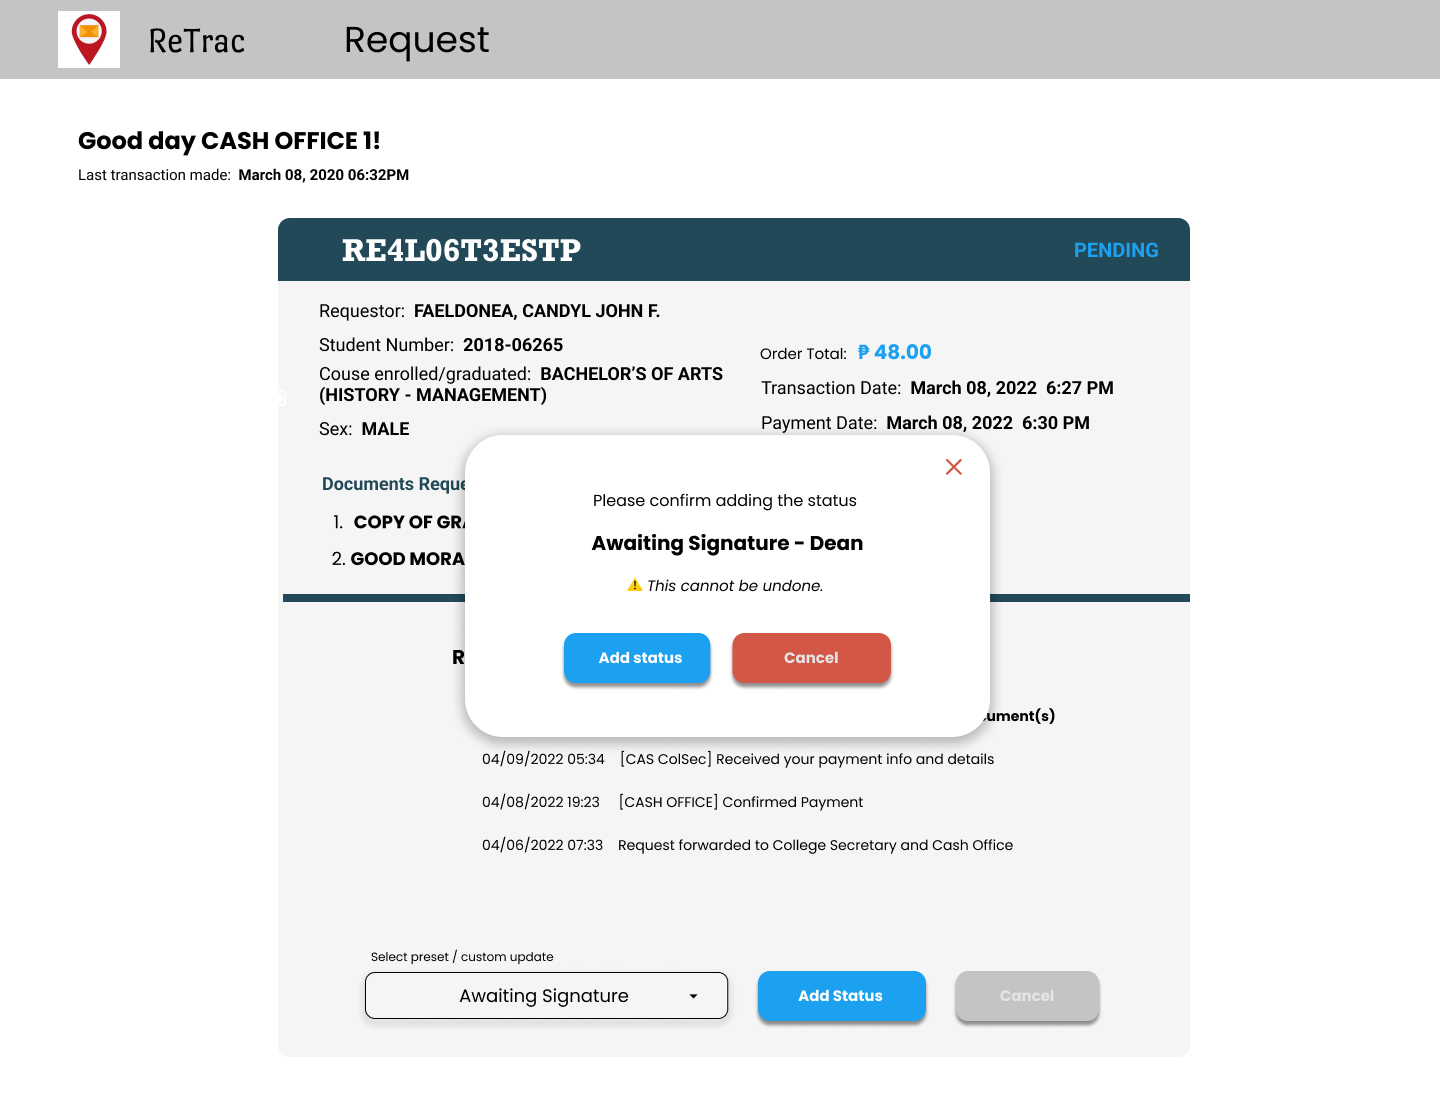
\includegraphics[width=0.9\columnwidth]{CS_Request4.png}
        \caption{Status update prompt}
        \label{fig:CS_Request4}
    \end{minipage}
\end{figure}

The check and status page will be a single page directed when the request status is marked as new or pending. The office can add request status such as “for approval by the dean”, “awaiting signature”, and custom update. In case the secretary wants to upload the file requested, it will then proceed to the file upload page where the office can upload multiple PDF, JPEG, and PNG files.

\begin{figure}[h]
    \centering 
    \begin{minipage}[c]{0.5\linewidth}
        \centering
        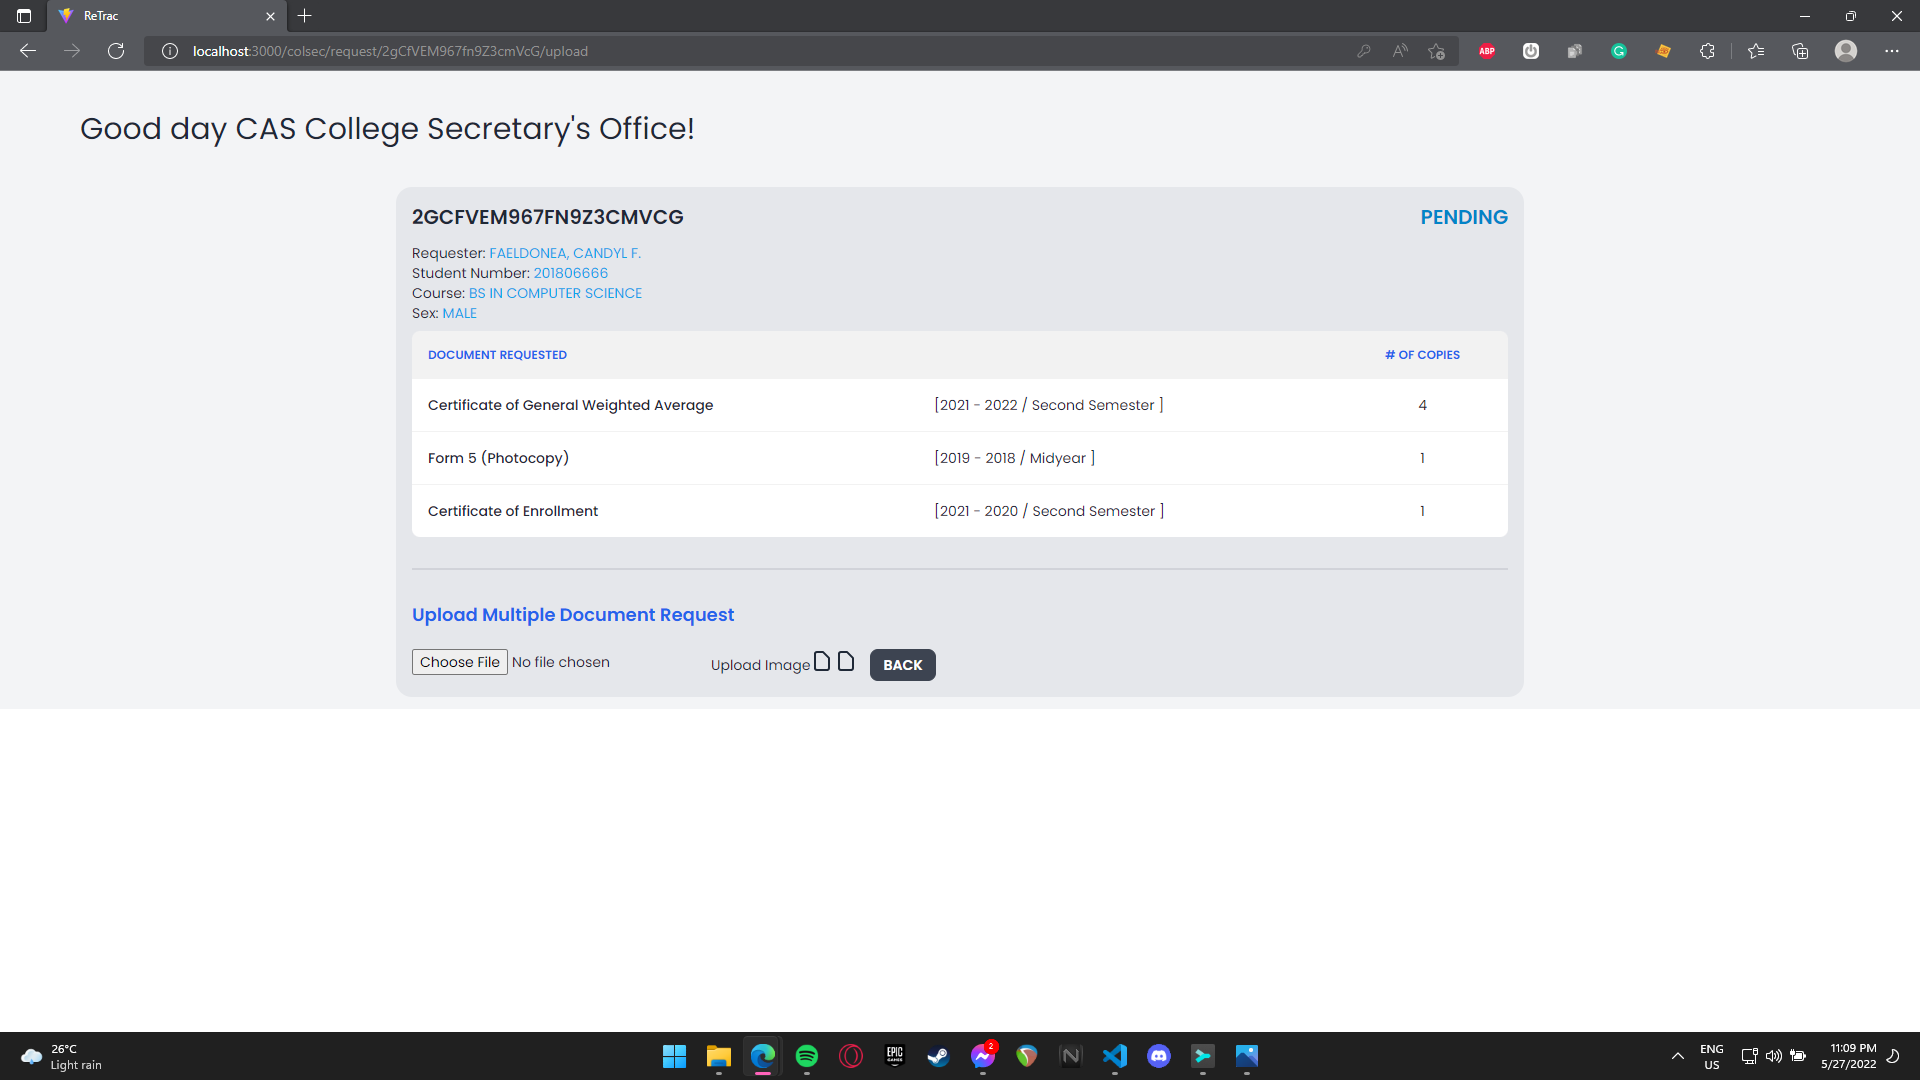
\includegraphics[width=0.9\columnwidth]{CS_Request3.png}
        \caption{Multiple files uploading bin}
        \label{fig:CS_Request3}
    \end{minipage}
\end{figure}

\begin{figure}[h]
    \centering 
    \begin{minipage}[c]{0.5\linewidth}
        \centering
        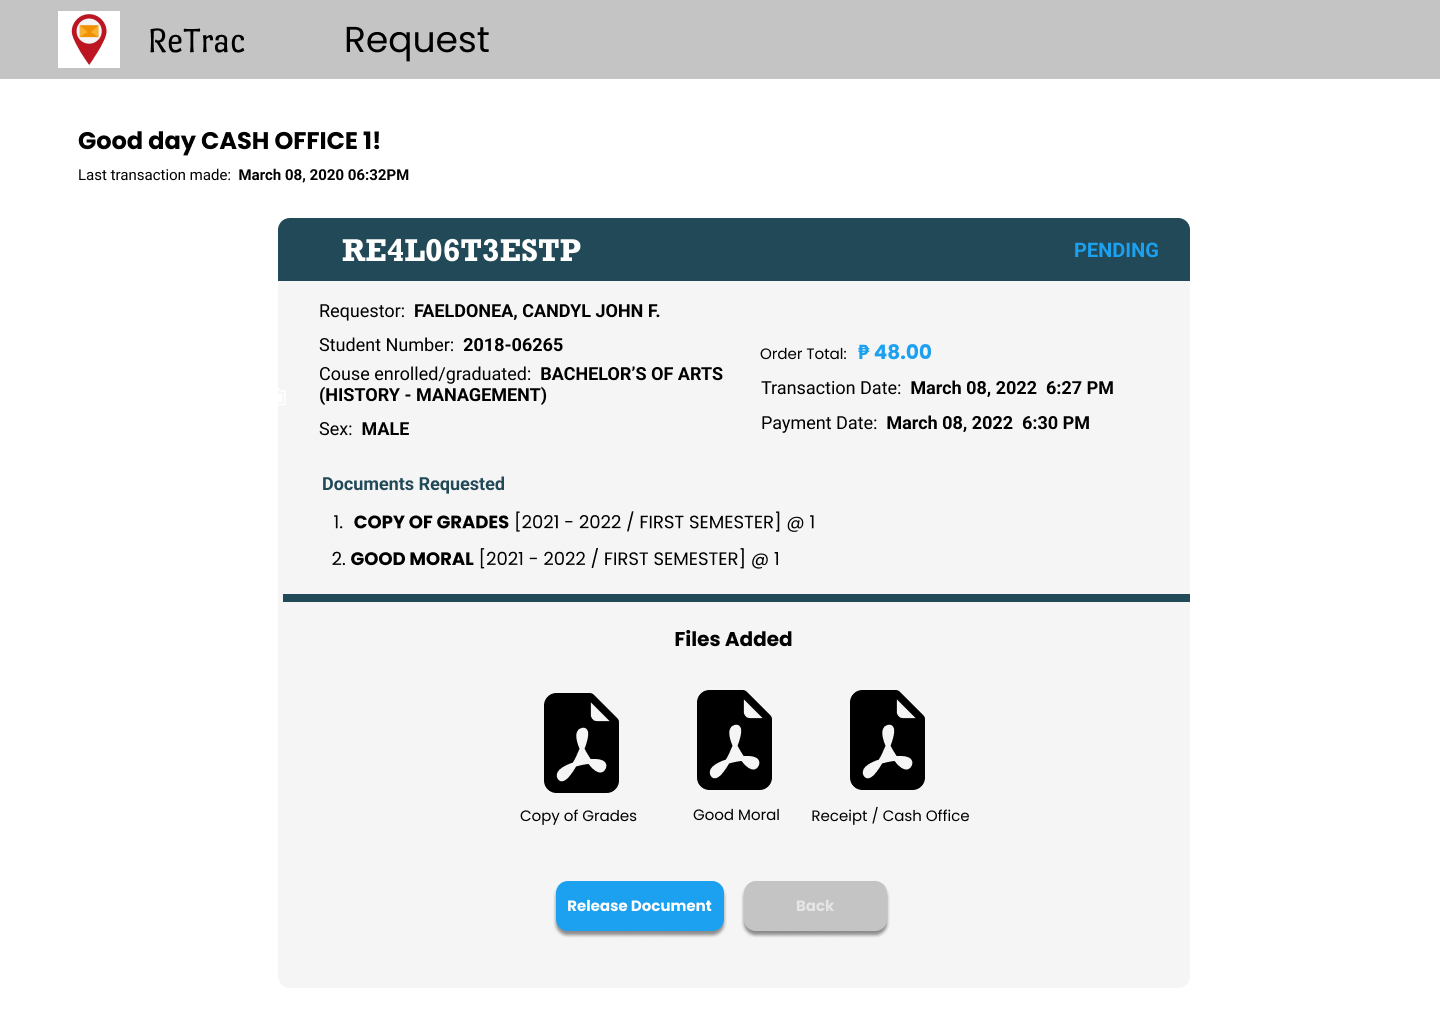
\includegraphics[width=0.9\columnwidth]{CS_Request5.png}
        \caption{File preview and releasing page}
        \label{fig:CS_Request5}
    \end{minipage}
\end{figure}

The office view will then display the file releasing page where it previews the files uploaded. The OR received from the cash office will automatically be added to the file pool the user can download. Pressing the “Release Document” will mark the document/s as “released” and will let the user access the document/s.

\subsubsection{Request History}

The last view of the college secretary\textsc{\char13}s office will aid them in documenting report as well as monitoring the requests that go in and out of their offices.

\begin{figure}[h]
    \centering 
    \begin{minipage}[c]{0.5\linewidth}
        \centering
        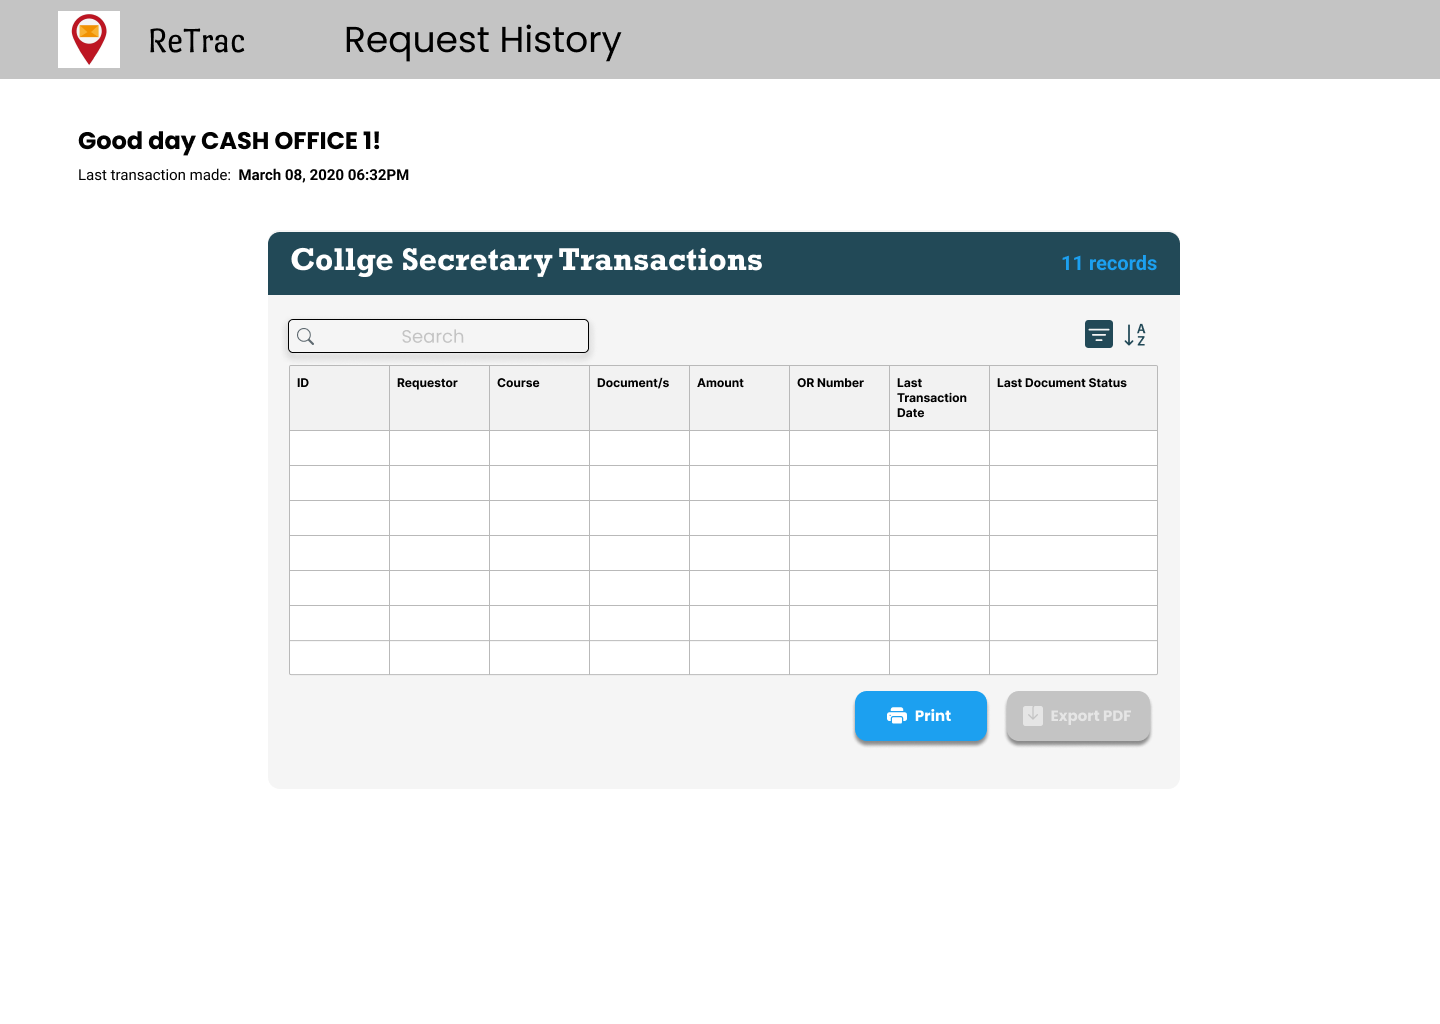
\includegraphics[width=0.9\columnwidth]{CS_RequestHistory.png}
        \caption{Read-only request history page}
        \label{fig:CS_RequestHistory}
    \end{minipage}
\end{figure}

The Request History page will feature a table report where the office can either print or export the tables as a PDF file. It has sorting and search features. However, this table will be read-only for monitoring and report purposes. This will give the office a quick glance at the transactions including those archived.

\section{Analysis}
    \begin{figure}[h]
        \centering 
        \begin{minipage}[c]{0.7\linewidth}
            \centering
            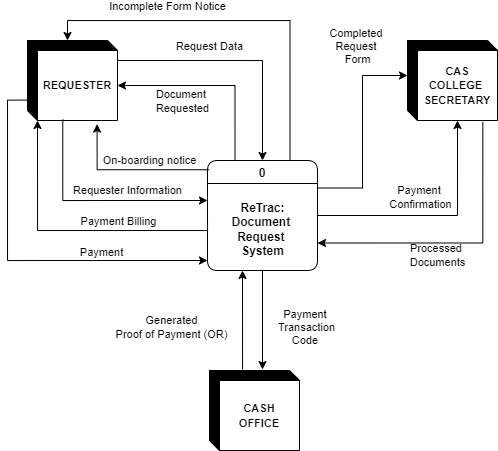
\includegraphics[width=0.9\columnwidth]{ContextDiagram.png}
            \caption{Context Diagram of the request system}
            \label{fig:ContextDiagra}
        \end{minipage}
    \end{figure}
    
    \begin{figure}[h]
        \centering 
        \begin{minipage}[c]{0.7\linewidth}
            \centering
            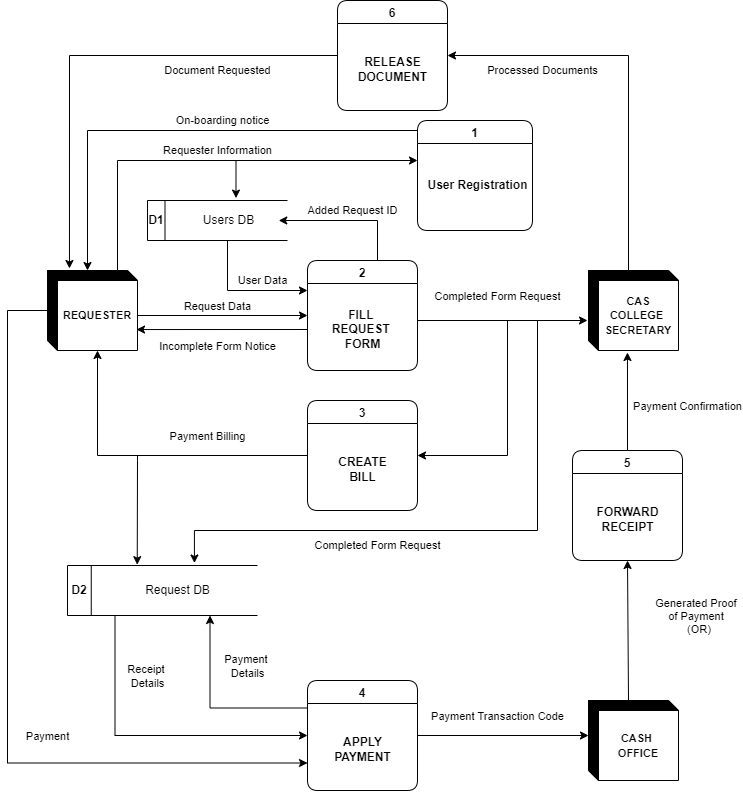
\includegraphics[width=0.9\columnwidth]{Diagram0.png}
            \caption{Diagram Level 0 of the request system}
            \label{fig:Diagram0}
        \end{minipage}
    \end{figure}
    
The context diagram shows the general functions of the system and the entities that our system is communicating with.



\section{Discussions}

This system allows the requestor to request student documents from the College of Arts and Sciences College Secretary. The web application works at optimum in a desktop environment and is designed to step-by-step process or minimize clicks and touch on some of its components. The User Interface and Experience are both designed to utilize less data and storage by minimizing rasterized images and implementing a minimalist approach similar to current systems used in UPV. In this study, the researchers are yet to implement an automated online banking payment method. However, this will be added in the recommendation section of this paper and will be implemented in some updates in the future.

As shown in the results section of this paper, the developers were able to implement the core components of the web application and its functionalities: sign in and sign up, dashboard access, request forms, payment portal, tracking page, and various office functionalities such as payment verification and request status update. Each of the mentioned functionalities and features was implemented based on the review of related literature and methodology. 

A portion of the web application is currently available thru local access backed with firebase remotely. Currently, it is in the internal debugging and testing phase.



